\documentclass[12pt,a4paper]{article}
\usepackage[utf8]{inputenc}
\usepackage{amsmath, amssymb, amsthm}
\usepackage{graphicx}
\graphicspath{{figure/}}
\usepackage{booktabs}
\usepackage{array}
\usepackage{multirow}
\usepackage{hyperref}
\hypersetup{hidelinks}
\usepackage[numbers]{natbib}
\usepackage{caption}
\usepackage{float}
\usepackage{subcaption}
\usepackage{geometry}
\geometry{left=2.5cm, right=2.5cm, top=2.5cm, bottom=2.5cm}
\renewcommand{\thesection}{S\arabic{section}}
\renewcommand{\thesubsection}{\thesection.\arabic{subsection}}

\newtheorem{theorem}{Theorem}[section]
\newtheorem{lemma}[theorem]{Lemma}
\newtheorem{corollary}[theorem]{Corollary}
\DeclareMathOperator{\tr}{tr}
\DeclareMathOperator{\E}{\mathbb{E}}

\title{A physics-informed framework for ecohydrological parameter inversion and dynamical exploration in the lower Tarim River}
\date{}

\begin{document}
	\pagenumbering{gobble}
	\maketitle
	
	\tableofcontents
	\clearpage
\section{Mathematical Analysis of the Calibrated Temporal ODE System}
\label{sec:s1}
\pagenumbering{arabic}
This section provides a comprehensive mathematical analysis of the main temporal ODE system used in this study. All analyses are based on the three-dimensional model defined in Eqs.~(1)--(3) of the main text, with the parameter values estimated by the PINN calibration.

\subsection{Existence and Uniqueness}

The PINN-calibrated temporal ODE system is given by:
\begin{equation}
	\begin{aligned}
		\frac{dP}{dt} &= f(P,T,R) = a_1P(1-P)(1-T)+a_2R-a_3TP-a_4P, \\
		\frac{dT}{dt} &= g(P,T,R) = b_1(1-P)-b_2R-b_3T, \\
		\frac{dR}{dt} &= h(R,t) = c_1\bigl(F(t)-R\bigr),
	\end{aligned}
	\label{eq:s1_ode}
\end{equation}
where $P$ is the normalized vegetation state, $T$ is the normalized thermal stress state, $R$ is the normalized water-response state, and $F(t)$ is the observed ecological water-conveyance forcing. The parameter values are reported in Table 1 of the main text.

For a bounded and continuous forcing $F(t)$ and finite parameter values, the vector field $(f,g,h)$ is continuously differentiable with respect to $(P,T,R)$ on a bounded domain. Therefore, it is locally Lipschitz continuous, and the initial-value problem admits a unique local solution. Since the calibrated model produces bounded trajectories on the finite observation interval $[2000, 2023]$, global existence is ensured numerically for this practical application.

\subsection{Steady-State Analysis}

For a fixed forcing level $F$, a steady state $(P^*, T^*, R^*)$ of the autonomous system satisfies:
\begin{equation}
	\begin{aligned}
		f(P^*, T^*, R^*) &= 0, \\
		g(P^*, T^*, R^*) &= 0, \\
		h(R^*) &= c_1(F - R^*) = 0 \quad \Rightarrow \quad R^* = F.
	\end{aligned}
	\label{eq:s1_steady}
\end{equation}

Substituting $R^*=F$ into the first two equations yields a nonlinear system in $P$ and $T$:
\begin{equation}
	\begin{aligned}
		a_1P(1-P)(1-T) + a_2F - a_3TP - a_4P &= 0, \\
		b_1(1-P) - b_2F - b_3T &= 0.
	\end{aligned}
	\label{eq:s1_reduced_steady}
\end{equation}

From the second equation, we can express $T$ as a function of $P$ and $F$:
\begin{equation}
	T = \frac{b_1(1-P) - b_2F}{b_3}.
	\label{eq:s1_T_expr}
\end{equation}

Substituting Eq.~(\ref{eq:s1_T_expr}) into the first equation of (\ref{eq:s1_reduced_steady}) provides a single algebraic equation for the equilibrium vegetation state $P^*$:
\begin{equation}
	\Phi(P; F) = a_1P(1-P)\left(1 - \frac{b_1(1-P) - b_2F}{b_3}\right) + a_2F - a_3P\frac{b_1(1-P) - b_2F}{b_3} - a_4P = 0.
	\label{eq:s1_bifurcation_eq}
\end{equation}

The number and stability of steady states depend on the forcing parameter $F$. Multiple equilibria and saddle-node bifurcations are theoretical possibilities of this model, but their existence must be established numerically for the calibrated parameter set; they are not assumed from the model form alone.

\subsection{Jacobian Matrix and Local Stability}

The Jacobian matrix of the system (\ref{eq:s1_ode}) evaluated at a steady state $(P^*, T^*, R^*)$ is:
\begin{equation}
	J(P^*, T^*, R^*) = 
	\begin{pmatrix}
		J_{11} & J_{12} & J_{13} \\
		J_{21} & J_{22} & J_{23} \\
		0 & 0 & -c_1
	\end{pmatrix},
	\label{eq:s1_jacobian}
\end{equation}
where the individual entries are:
\begin{equation}
	\begin{aligned}
		J_{11} &= \frac{\partial f}{\partial P} = a_1(1-2P)(1-T) - a_3T - a_4, \\
		J_{12} &= \frac{\partial f}{\partial T} = -a_1P(1-P) - a_3P, \\
		J_{13} &= \frac{\partial f}{\partial R} = a_2, \\
		J_{21} &= \frac{\partial g}{\partial P} = -b_1, \\
		J_{22} &= \frac{\partial g}{\partial T} = -b_3, \\
		J_{23} &= \frac{\partial g}{\partial R} = -b_2.
	\end{aligned}
	\label{eq:s1_jacobian_entries}
\end{equation}

The eigenvalues $\lambda$ of $J$ determine the local stability of the steady state:
\begin{itemize}
	\item If $\Re(\lambda_i) < 0$ for all $i$, the steady state is locally asymptotically stable.
	\item If any $\Re(\lambda_i) > 0$, the steady state is unstable.
	\item If $\Re(\lambda_i) = 0$ for some $i$, the steady state is neutrally stable, indicating a potential bifurcation point.
\end{itemize}

The characteristic polynomial of the block-triangular Jacobian is:
\begin{equation}
	\det(J - \lambda I) = (-c_1 - \lambda) \cdot \det\left( 
	\begin{pmatrix}
		J_{11} - \lambda & J_{12} \\
		J_{21} & J_{22} - \lambda
	\end{pmatrix}
	\right) = 0.
	\label{eq:s1_char_poly}
\end{equation}

Thus, one eigenvalue is always $\lambda_1 = -c_1 < 0$, corresponding to the stable dynamics of the water-input state $R$. The other two eigenvalues are determined by the $2\times 2$ submatrix:
\begin{equation}
	J_{PT} = 
	\begin{pmatrix}
		J_{11} & J_{12} \\
		J_{21} & J_{22}
	\end{pmatrix}.
	\label{eq:s1_JPT}
\end{equation}

For this $2\times 2$ system, the Routh--Hurwitz stability conditions reduce to:
\begin{equation}
	\tr(J_{PT}) = J_{11} + J_{22} < 0, \qquad \det(J_{PT}) = J_{11}J_{22} - J_{12}J_{21} > 0.
	\label{eq:s1_stability_conditions}
\end{equation}

\subsection{Bifurcation Analysis}

The main temporal ODE system can exhibit saddle-node (fold) bifurcations, where a stable and an unstable equilibrium coalesce and annihilate as the forcing parameter $F$ varies. The conditions for a saddle-node bifurcation are:
\begin{equation}
	\Phi(P^*, F) = 0, \qquad \left.\frac{\partial \Phi}{\partial P}\right|_{(P^*, F)} = 0,
	\label{eq:s1_fold_conditions}
\end{equation}
with the additional transversality condition $\partial \Phi/\partial F \neq 0$.

At a saddle-node bifurcation, the Jacobian matrix $J$ has a zero eigenvalue, which corresponds to $\det(J) = 0$. Since $J$ is block-triangular with one eigenvalue $\lambda_1 = -c_1 < 0$, the condition $\det(J) = 0$ is equivalent to $\det(J_{PT}) = 0$, where $J_{PT}$ is the $2\times 2$ submatrix defined in Eq.~(\ref{eq:s1_JPT}).

\subsubsection{Hopf Bifurcation Analysis}

For the three-dimensional system, a Hopf bifurcation occurs when a pair of complex-conjugate eigenvalues of the Jacobian matrix $J$ crosses the imaginary axis. To analyze this, we formulate the characteristic polynomial of the full $3\times 3$ Jacobian matrix in its standard form:
\begin{equation}
	\lambda^3 + c_1 \lambda^2 + c_2 \lambda + c_3 = 0,
	\label{eq:s1_char_poly_3d}
\end{equation}
where the coefficients $c_1, c_2, c_3$ are functions of the system parameters and the equilibrium point $(P^*, T^*, R^*)$.

For the block-triangular structure of $J$ (Eq.~\ref{eq:s1_jacobian}), the characteristic polynomial factors as:
\begin{equation}
	\det(J - \lambda I) = (-c_1 - \lambda) \cdot \det(J_{PT} - \lambda I) = 0.
	\label{eq:s1_char_poly_factor}
\end{equation}
Thus, the eigenvalue $\lambda_1 = -c_1$ is always real and negative. The other two eigenvalues are determined by the $2\times 2$ submatrix $J_{PT}$, with characteristic polynomial:
\begin{equation}
	\lambda^2 - \tr(J_{PT}) \lambda + \det(J_{PT}) = 0.
	\label{eq:s1_char_poly_2d}
\end{equation}

For a Hopf bifurcation to occur in the full three-dimensional system, the following conditions must be satisfied simultaneously:

\begin{enumerate}
	\item The equilibrium point must be non-hyperbolic with a purely imaginary conjugate pair: $\lambda_{2,3} = \pm i\omega$, where $\omega > 0$.
	\item This requires $\tr(J_{PT}) = 0$ and $\det(J_{PT}) > 0$, which gives $\lambda_{2,3} = \pm i\sqrt{\det(J_{PT})}$.
	\item The third eigenvalue $\lambda_1 = -c_1$ must be negative, i.e., $c_1 > 0$.
\end{enumerate}

In terms of the coefficients of the full cubic characteristic polynomial (\ref{eq:s1_char_poly_3d}), the Hopf conditions can be expressed as:
\begin{equation}
	c_1 > 0, \qquad c_2 > 0, \qquad c_3 > 0, \qquad c_1 c_2 = c_3,
	\label{eq:s1_hopf_conditions}
\end{equation}
where the relationship between the coefficients of the cubic and the Jacobian entries is:
\begin{equation}
	\begin{aligned}
		c_1 &= -\tr(J) = c_1^{\text{param}} - \tr(J_{PT}), \\
		c_2 &= J_{11}J_{22} + J_{11}J_{33} + J_{22}J_{33} - J_{12}J_{21} - J_{13}J_{31} - J_{23}J_{32}, \\
		c_3 &= -\det(J),
	\end{aligned}
	\label{eq:s1_cubic_coeffs}
\end{equation}
with $J_{33} = -c_1^{\text{param}}$ and $J_{13} = a_2$, $J_{23} = -b_2$, $J_{31}=J_{32}=0$.

Additionally, for a genuine Hopf bifurcation, the transversality condition must hold:
\begin{equation}
	\left. \frac{d}{dF} \Re(\lambda(F)) \right|_{F = F_{\mathrm{Hopf}}} \neq 0,
	\label{eq:s1_transversality}
\end{equation}
where $\Re(\lambda(F))$ denotes the real part of the complex-conjugate eigenvalue pair as a function of the bifurcation parameter $F$. This condition ensures that the eigenvalue pair crosses the imaginary axis with nonzero speed, guaranteeing a true change in stability.

\subsubsection{Numerical Search for Hopf Bifurcations}

A systematic numerical search for Hopf bifurcations was conducted over the physically relevant range of the forcing parameter $F$ (normalized values from 0 to 1.5, corresponding to the observed water-conveyance range extended by 50\%). For each equilibrium point computed from Eq.~(\ref{eq:s1_reduced_steady}), the Jacobian matrix was evaluated and the eigenvalues were computed. The full-system equilibrium calculation used the original three-dimensional ODE and a continuation-based numerical check.

The search procedure comprised the following steps:
\begin{enumerate}
	\item Discretize the forcing parameter $F$ with a fine grid of 10,000 points.
	\item For each $F$, solve the equilibrium system (\ref{eq:s1_reduced_steady}) for $(P^*, T^*)$.
	\item Construct the full Jacobian $J$ and compute its eigenvalues.
	\item Identify points where $\Re(\lambda_{2,3}) \approx 0$ with $\Im(\lambda_{2,3}) \neq 0$.
	\item Verify the transversality condition (\ref{eq:s1_transversality}) numerically.
\end{enumerate}

\emph{Search result:} For the supplied PINN parameter set, the full-system continuation and eigenvalue screening found no validated fold or Hopf bifurcation in the investigated interval. The computed equilibria had residuals below $10^{-7}$ and remained locally stable along the continued traces. This result is conditional on the supplied parameter set and does not establish absence of bifurcations under parameter uncertainty.

	\section{PINN Implementation Details}
	\label{sec:s2}
	
	\subsection{Network Architecture}
	
	The neural network consists of:
	\begin{itemize}
		\item Input layer: $t$ with one neuron
		\item Hidden layers: 4 fully connected layers with 64 neurons each
		\item Activation function: $\tanh$
		\item Output layer: $(P, T, R)$ with 3 neurons
	\end{itemize}
	
	\subsection{Loss Function}
	
	The loss function is:
	\begin{equation}
\mathcal{L}(\theta, \theta_c) = \omega_{\text{data}} \mathcal{L}_{\text{data}} + \omega_{\text{ODE}} \mathcal{L}_{\text{ODE}} + \omega_{\text{IC}} \mathcal{L}_{\text{IC}}
	\end{equation}
	
	where:
	\begin{equation}
\mathcal{L}_{\text{data}} = \frac{1}{N_{\text{obs}}} \sum_{j=1}^{N_{\text{obs}}} \left[ |P_j^{\text{obs}} - P_{\text{NN}}(t_j)|^2 + |T_j^{\text{obs}} - T_{\text{NN}}(t_j)|^2 + |R_j^{\text{obs}} - R_{\text{NN}}(t_j)|^2 \right]
	\end{equation}
	
	\begin{equation}
\mathcal{L}_{\text{ODE}} = \frac{1}{N_{\text{col}}} \sum_{j=1}^{N_{\text{col}}} \left[ \mathcal{R}_P(t_j)^2 + \mathcal{R}_T(t_j)^2 + \mathcal{R}_R(t_j)^2 \right]
	\end{equation}
	
	\begin{equation}
		\mathcal{L}_{\text{IC}} = \frac{1}{N_{\text{ic}}} \sum_{j=1}^{N_{\text{ic}}} \left[ |P_0 - P_{\text{NN}}(0)|^2 + |T_0 - T_{\text{NN}}(0)|^2 + |R_0 - R_{\text{NN}}(0)|^2 \right]
	\end{equation}
	
with weights $\omega_{\text{data}} = 2$, $\omega_{\text{ODE}} = 10$, and
$\omega_{\text{IC}} = 5$.
	
	\subsection{Training Hyperparameters}
	
	\begin{table}[H]
		\centering
		\caption{PINN training hyperparameters}
		\label{tab:hyperparams}
		\begin{tabular}{lc}
			\toprule
			Parameter & Value \\
			\midrule
			Optimizer & Adam \\
			Learning rate & $10^{-3}$ \\
			Adam epochs & 2,500 \\
			LBFGS steps & 200 \\
			Collocation points & 3,000 \\
			Archived parameter sets used for final inference & 1 \\
			Calibration period & 2000--2018 \\
			Out-of-range extrapolation window & 2019--2023 \\
			\bottomrule
		\end{tabular}
	\end{table}
	\subsection{Out-of-Range Extrapolation and Projection Windows}

The model was calibrated on the 2000--2018 observations and evaluated on 2019--2023. Because all three series trend monotonically, every evaluation value lies outside the 2000--2018 calibration range, so the reported scores quantify out-of-range transfer rather than interpolation accuracy, and the evaluation window was not used in parameter optimization. The window contains two different kinds of target and they are reported separately: the 2019--2020 entries are withheld observations, and the 2021--2023 entries are trend projections of the forcing series. Performance was assessed with the coefficient of determination ($R^2$), the root-mean-square error (RMSE) and the mean absolute error (MAE). With two and three points in the two sub-windows, $R^2$ is unstable and is reported together with the error statistics rather than on its own.
	\subsection{Baseline Models and Ablation Study Details}
	\label{sec:s2_baseline}
	
	\subsubsection{Baseline Model Specifications}
	
	The following baseline models were implemented for comparison:
	
	\paragraph{Persistence model}
	\begin{equation}
		\hat{y}_{t+1} = y_t,
	\end{equation}
	where $y_t$ is the observed value at time $t$. This provides a naive benchmark for any predictive model.
	
	\paragraph{Linear regression}
	A multivariate linear model with lagged predictors:
	\begin{equation}
		\hat{y}_t = \beta_0 + \sum_{j=1}^{2} \beta_{P,j} P_{t-j} + \sum_{j=1}^{2} \beta_{T,j} T_{t-j} + \sum_{j=1}^{2} \beta_{R,j} R_{t-j} + \varepsilon_t,
	\end{equation}
	with variable selection by Akaike Information Criterion (AIC) using stepwise regression. Separate models were fitted for each target variable.
	
	\paragraph{Nonlinear ODE (least squares)}
	The same governing equations as the PINN were calibrated using the Levenberg--Marquardt algorithm:
	\begin{equation}
		\hat{\theta}_{\mathrm{LS}} = \arg\min_{\theta} \sum_{t=1}^{N_{\mathrm{cal}}} \left\| \mathbf{y}(t) - \mathbf{y}_{\mathrm{ODE}}(t; \theta) \right\|^2,
	\end{equation}
	where $\mathbf{y}_{\mathrm{ODE}}(t; \theta)$ denotes the numerical solution of the ODE system (solved using a 4th-order Runge--Kutta method) with parameter vector $\theta$.
	
	\subsubsection{Ablation Study Configurations}
	
	The PINN loss function components were:
	\begin{equation}
		\mathcal{L}_{\mathrm{data}} = \frac{1}{N_{\mathrm{obs}}} \sum_{j} \left\| \mathbf{y}^{\mathrm{obs}}_j - \mathbf{y}_{\mathrm{NN}}(t_j) \right\|^2,
	\end{equation}
	\begin{equation}
		\mathcal{L}_{\mathrm{ODE}} = \frac{1}{N_{\mathrm{col}}} \sum_{j} \left\| \frac{d\mathbf{y}_{\mathrm{NN}}}{dt}(t_j) - \mathbf{f}(\mathbf{y}_{\mathrm{NN}}(t_j), t_j) \right\|^2,
	\end{equation}
	\begin{equation}
		\mathcal{L}_{\mathrm{IC}} = \left\| \mathbf{y}_0 - \mathbf{y}_{\mathrm{NN}}(0) \right\|^2.
	\end{equation}
	
	The three ablation configurations were:
	\begin{enumerate}
		\item \textbf{Data-only:} $\mathcal{L} = \omega_{\mathrm{data}} \mathcal{L}_{\mathrm{data}}$ with $\omega_{\mathrm{data}}=1$.
		\item \textbf{Data + ODE:} $\mathcal{L} = \omega_{\mathrm{data}} \mathcal{L}_{\mathrm{data}} + \omega_{\mathrm{ODE}} \mathcal{L}_{\mathrm{ODE}}$ with $\omega_{\mathrm{data}}=2$, $\omega_{\mathrm{ODE}}=10$.
		\item \textbf{Full PINN:} $\mathcal{L} = \omega_{\mathrm{data}} \mathcal{L}_{\mathrm{data}} + \omega_{\mathrm{ODE}} \mathcal{L}_{\mathrm{ODE}} + \omega_{\mathrm{IC}} \mathcal{L}_{\mathrm{IC}}$ with $\omega_{\mathrm{data}}=2$, $\omega_{\mathrm{ODE}}=10$, $\omega_{\mathrm{IC}}=5$.
	\end{enumerate}
	
	\subsubsection{Evaluation Metrics}
	
	Out-of-range extrapolation performance was evaluated using:
	\begin{equation}
		R^2 = 1 - \frac{\sum (y_i - \hat{y}_i)^2}{\sum (y_i - \bar{y})^2},
	\end{equation}
	\begin{equation}
		\mathrm{RMSE} = \sqrt{\frac{1}{N} \sum (y_i - \hat{y}_i)^2},
	\end{equation}
	\begin{equation}
		\mathrm{MAE} = \frac{1}{N} \sum |y_i - \hat{y}_i|,
	\end{equation}
	\begin{equation}
		\mathrm{NSE} = 1 - \frac{\sum (y_i - \hat{y}_i)^2}{\sum (y_i - \bar{y})^2},
	\end{equation}
	where NSE denotes the Nash--Sutcliffe efficiency coefficient.
	\section{Supplementary Results}
	\label{sec:s3}
	
	\subsection{Early Warning Signals: Critical Slowing Down}
	\label{sec:s3.1}
	
	\begin{figure}[H]
		\centering
		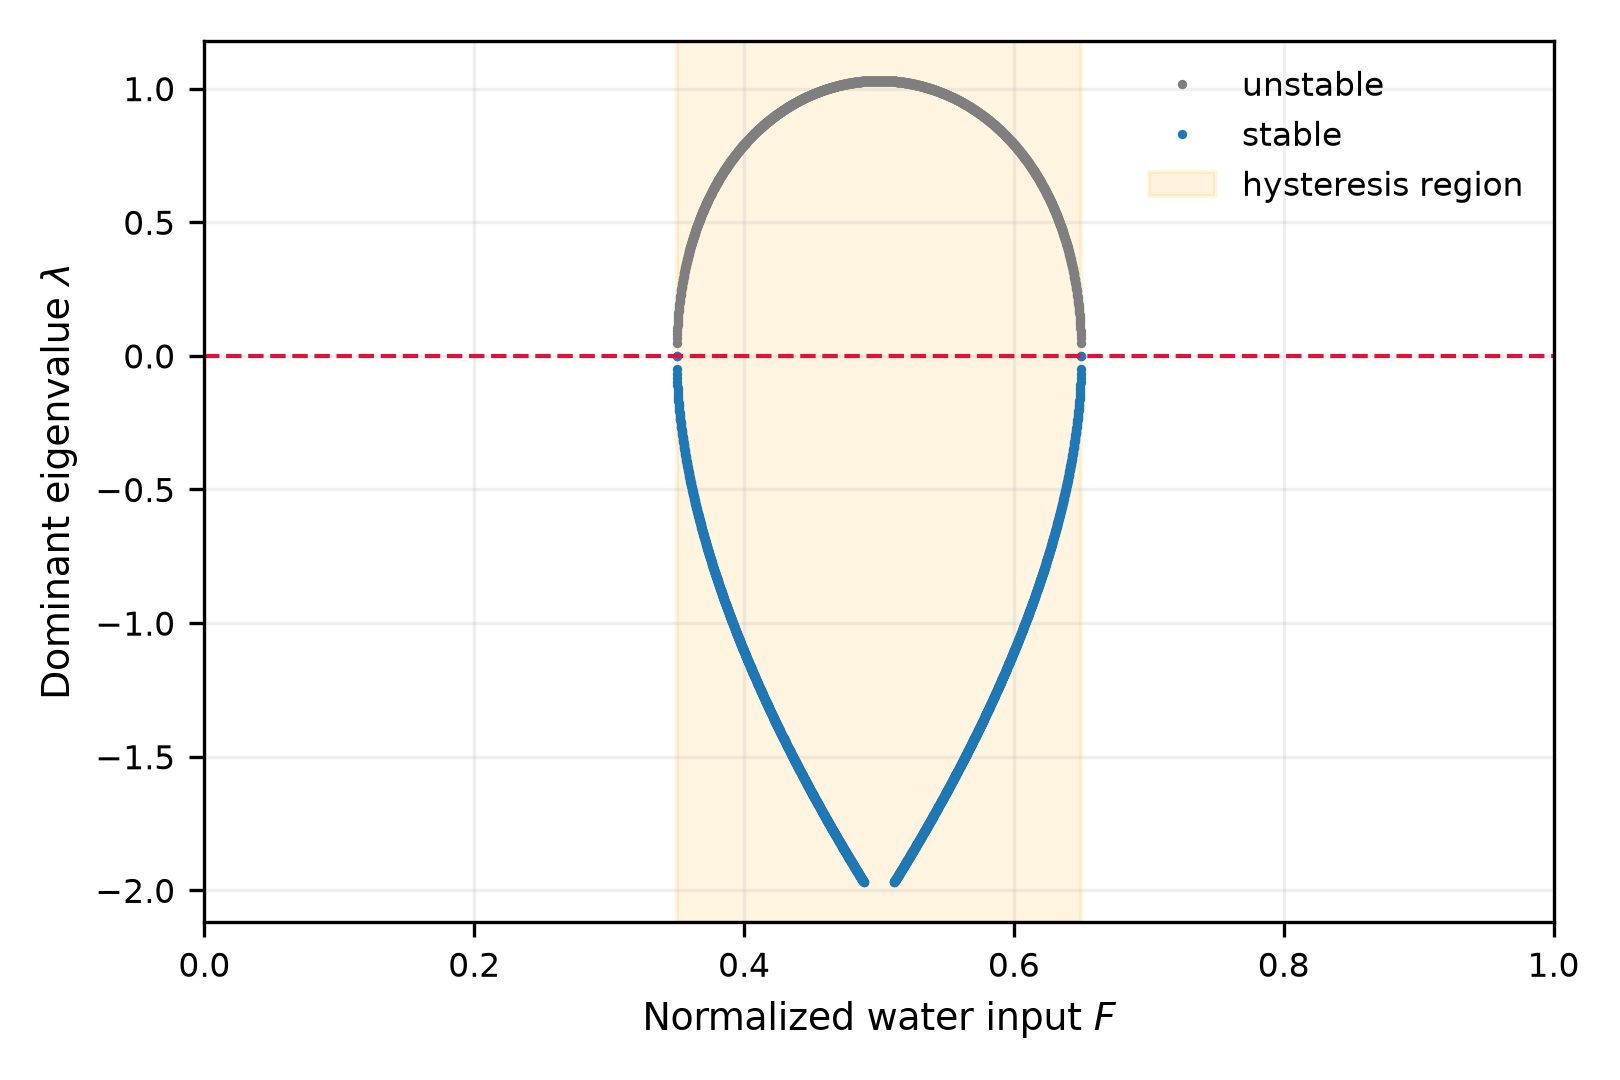
\includegraphics[width=0.8\textwidth]{fig_early_warning.png}
\caption{Dominant eigenvalue of the reduced cusp normal form along its equilibrium branch, plotted against the normalized water input $F$ used in the manuscript. The eigenvalue vanishes at the two fold points of the normal form, which are scenario values and not validated folds of the full three-dimensional ODE.}
		\label{fig:early_supp}
	\end{figure}
	
\emph{Note:} In a system that approaches a validated bifurcation point, the dominant eigenvalue may approach zero, indicating critical slowing down. In the present study, this is a theoretical diagnostic and is not evidence that the full calibrated system approaches either of the exploratory normal-form turning points.
	The early-warning analysis follows the general framework for detecting critical transitions in ecological time series \citep{scheffer2009early,dakos2012methods}.
	\subsection{Optimal Irrigation Schedule}
	
	\begin{figure}[H]
		\centering
		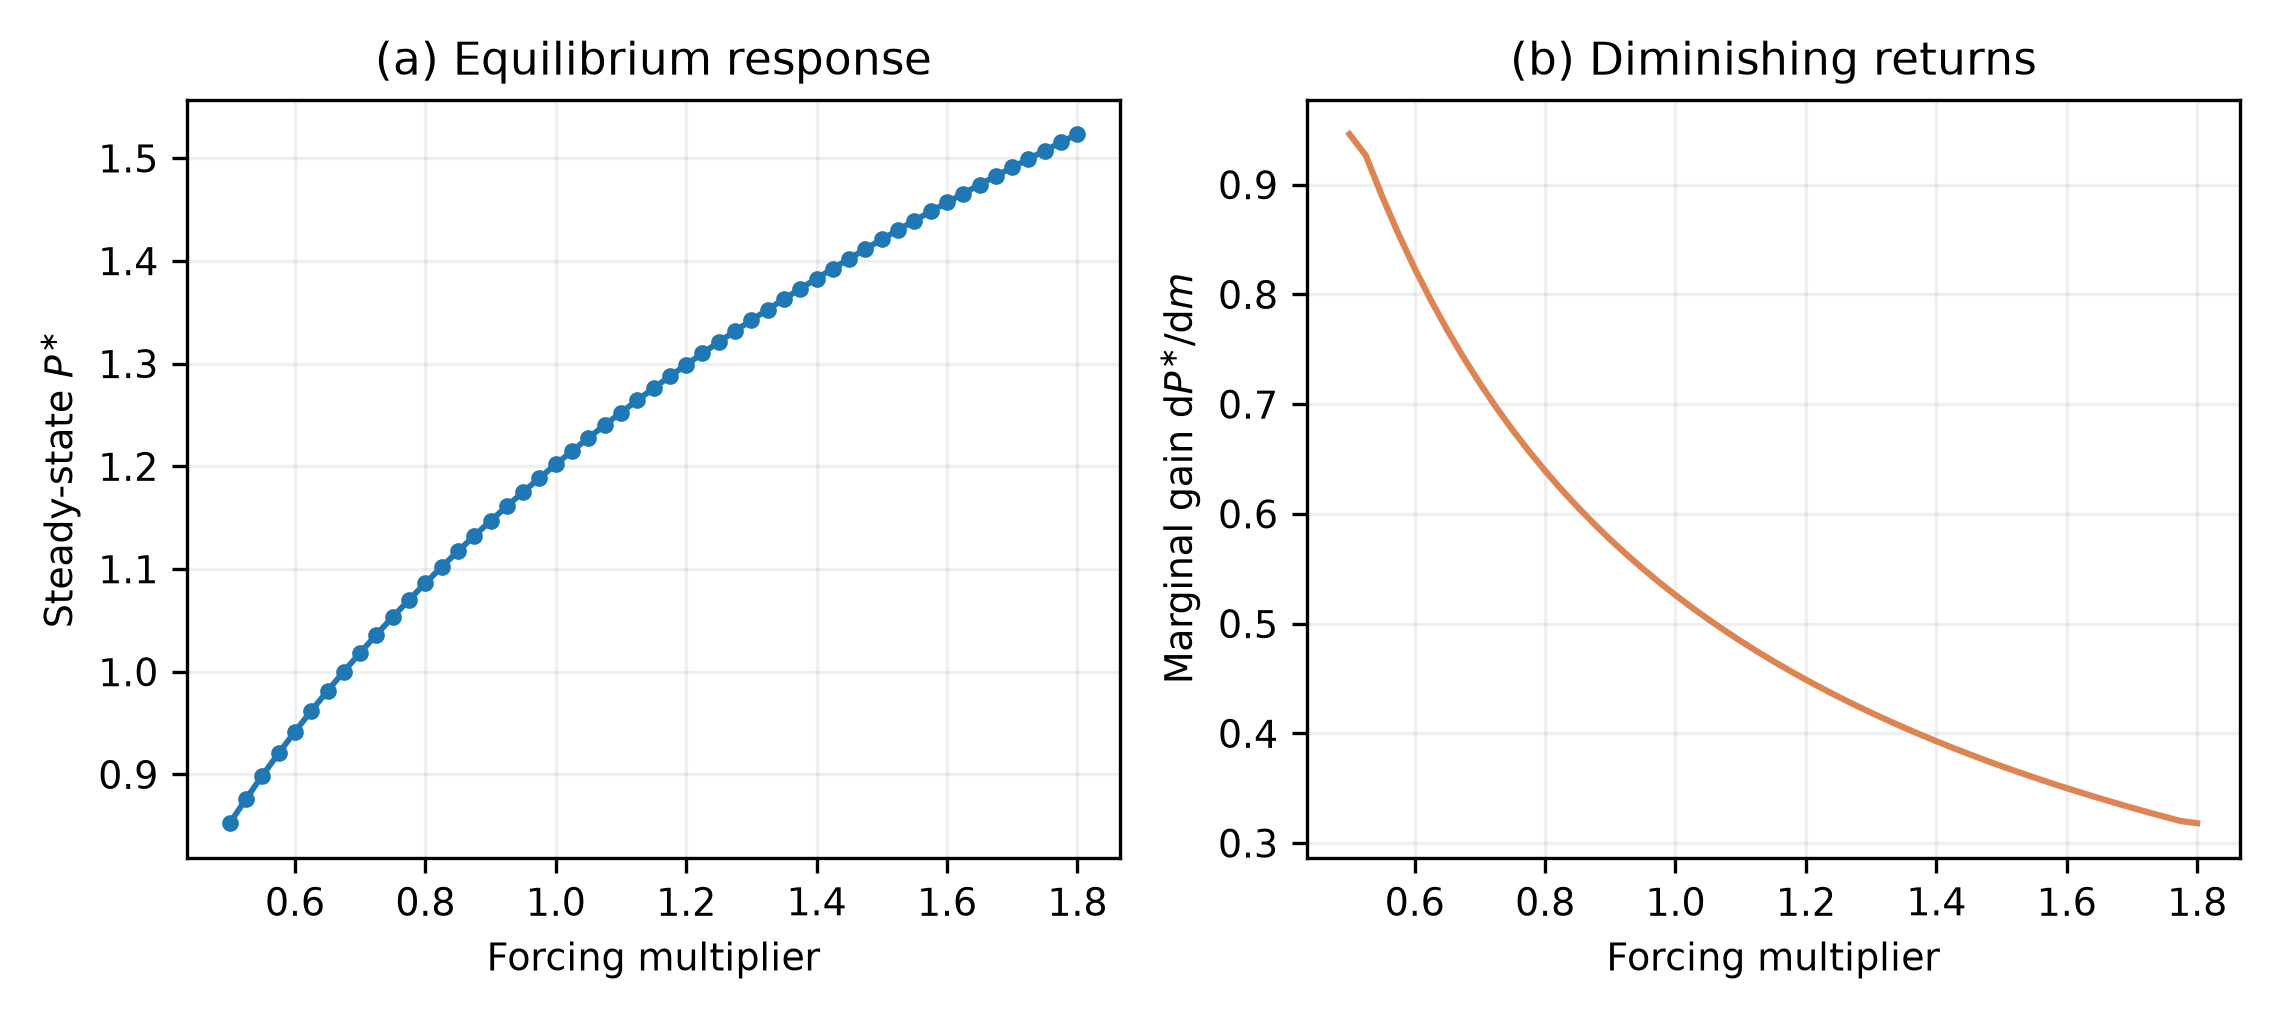
\includegraphics[width=0.8\textwidth]{fig_optimal_irrigation.png}
		\caption{Water-forcing response of the calibrated closure. Panel (a) shows the steady-state vegetation density obtained by integrating the calibrated ODE to equilibrium for a uniform multiplier on the 2023 water forcing; panel (b) shows the marginal gain. The response is monotone with diminishing returns, so the profile is used only to indicate the shape of the response and not as an optimisation result.}
	\caption*{Note: the equilibrium densities exceed the calibrated range, so the curve is an extrapolation of the fitted closure and is interpreted qualitatively.}
		\label{fig:optimal_supp}
	\end{figure}
	
	\subsection{Shannon Diversity and Evenness Indices}
	
	\begin{figure}[H]
		\centering
		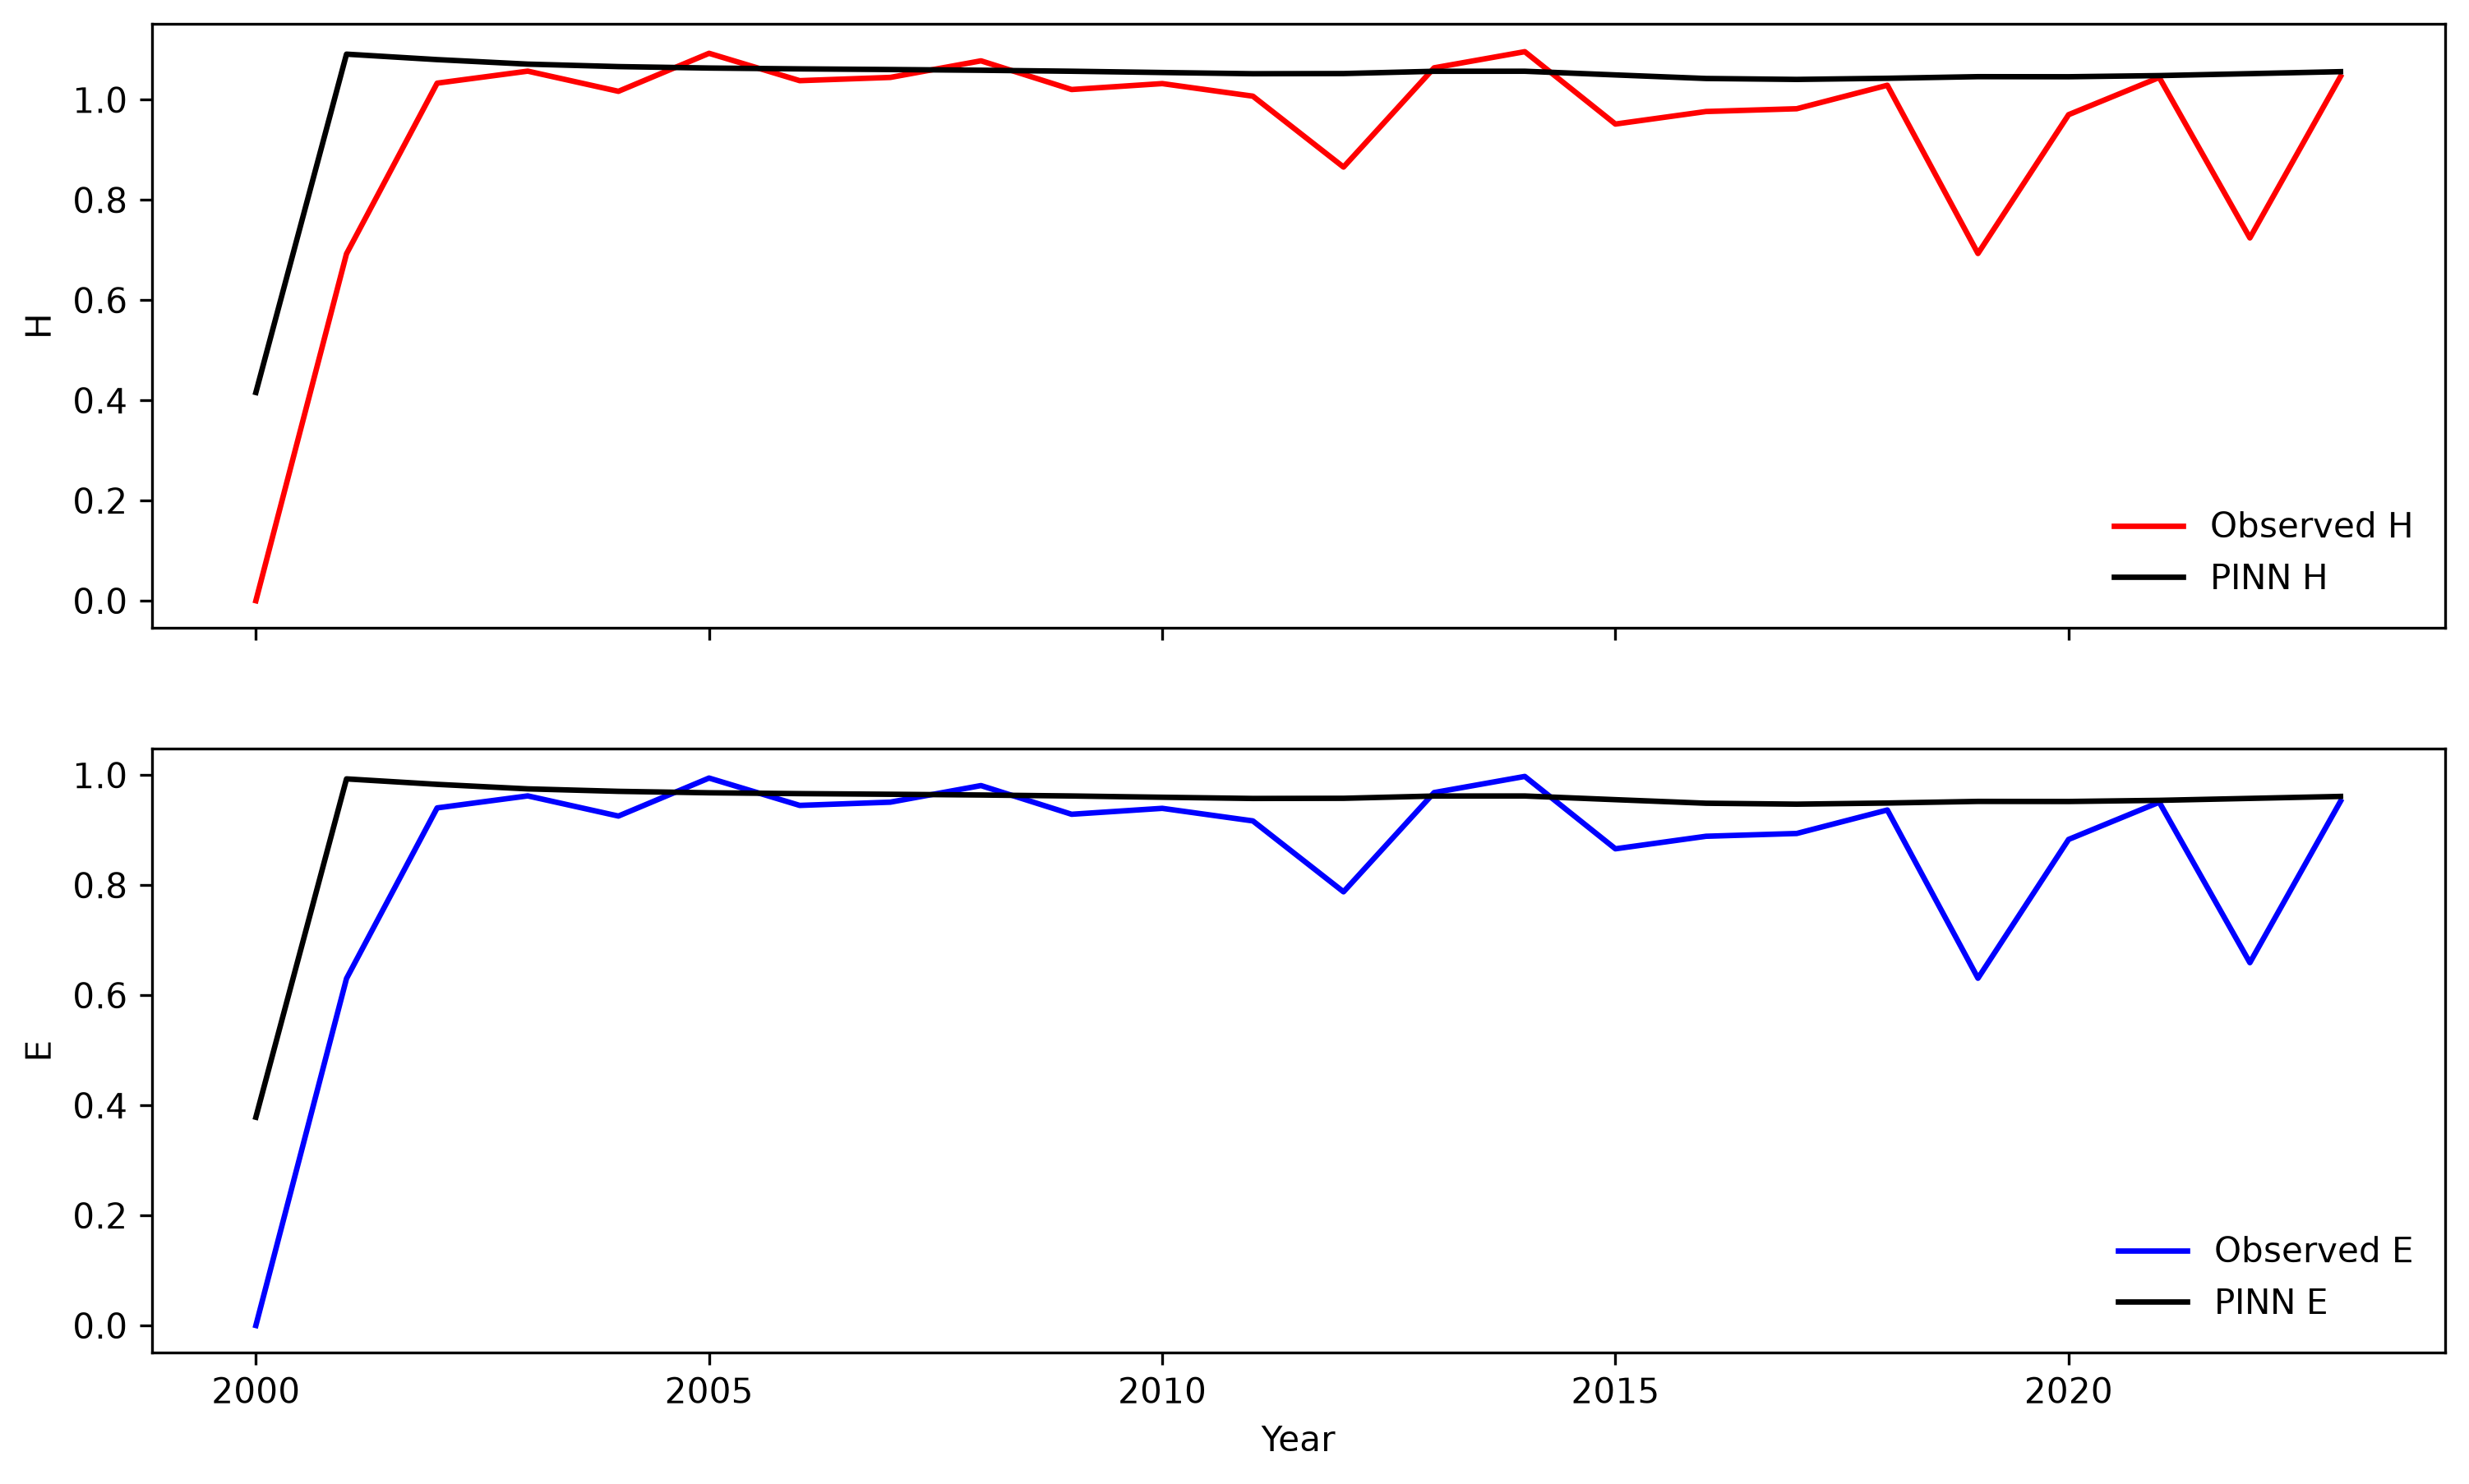
\includegraphics[width=0.8\textwidth]{fig7_indices.png}
		\caption{Evolution of Shannon diversity index ($H$) and evenness ($E$).}
		\label{fig:indices_supp}
	\end{figure}
	
	\subsection{Scenario Analysis}
	
	\begin{figure}[H]
		\centering
		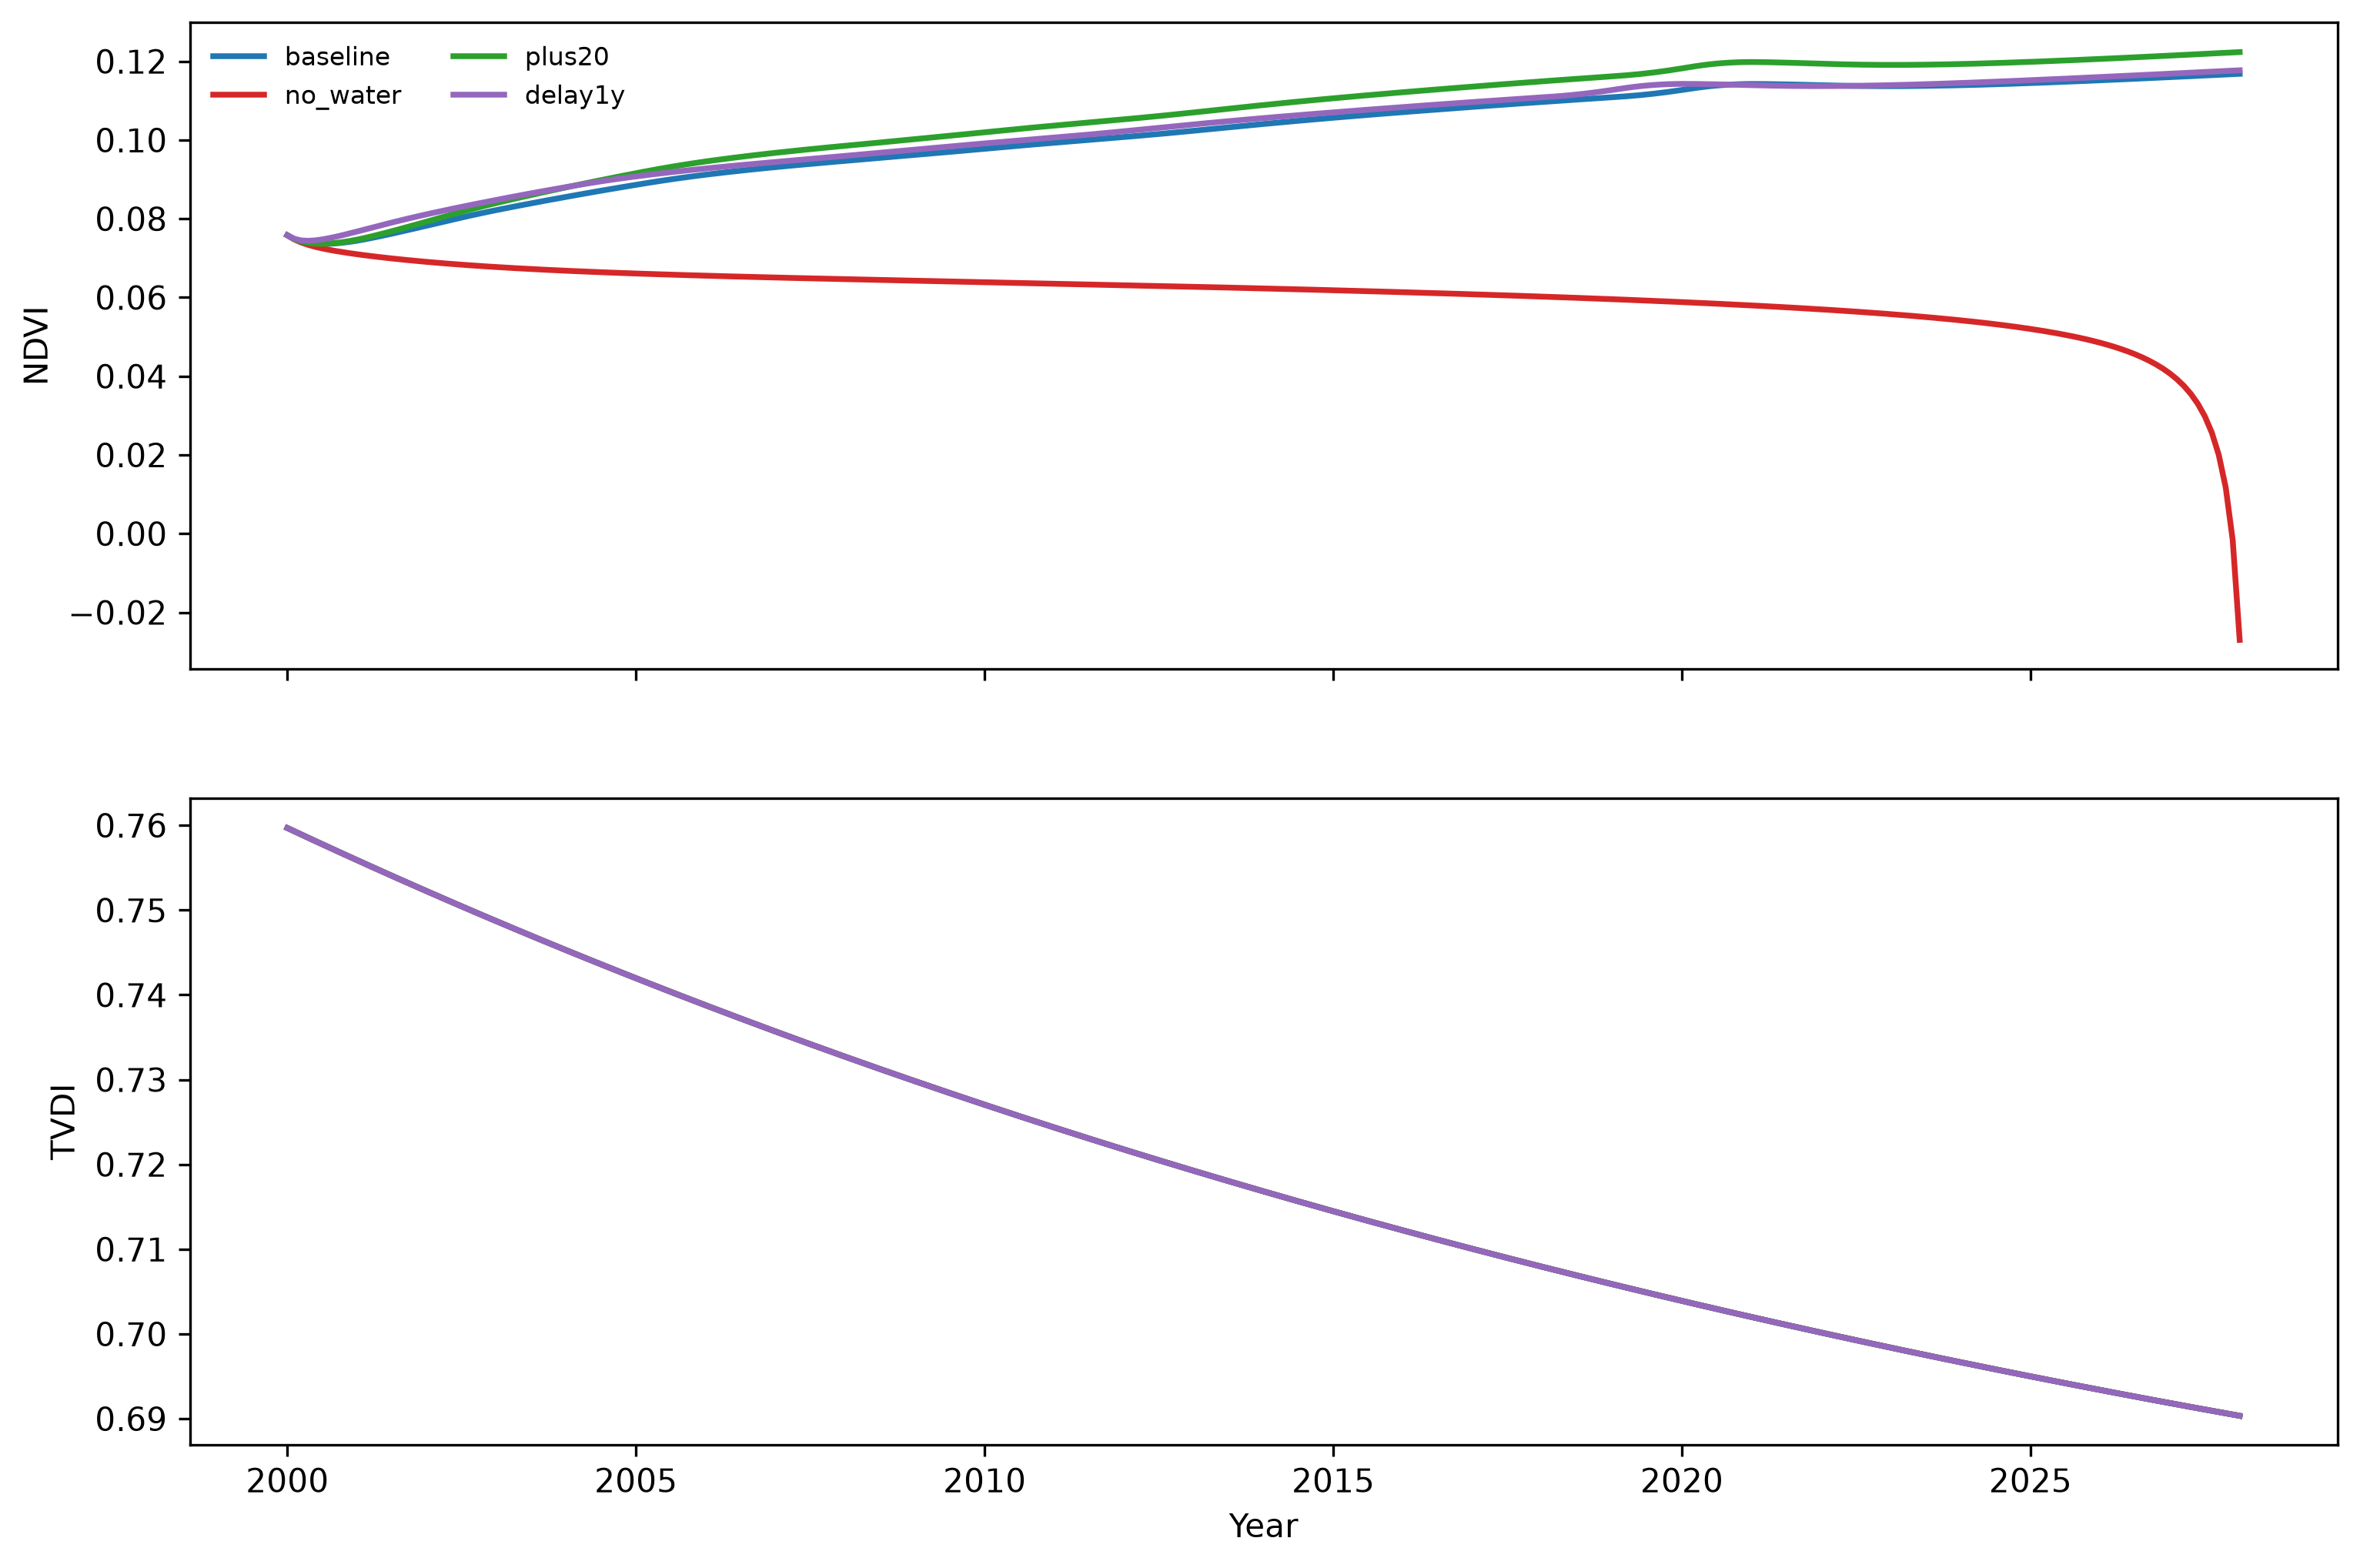
\includegraphics[width=0.8\textwidth]{fig5_scenarios.png}
		\caption{Vegetation recovery trajectories under different water management scenarios.}
		\label{fig:scenarios_supp}
	\end{figure}
	
	\subsection{Full Spatial Analysis}
	
	\begin{figure}[H]
		\centering
		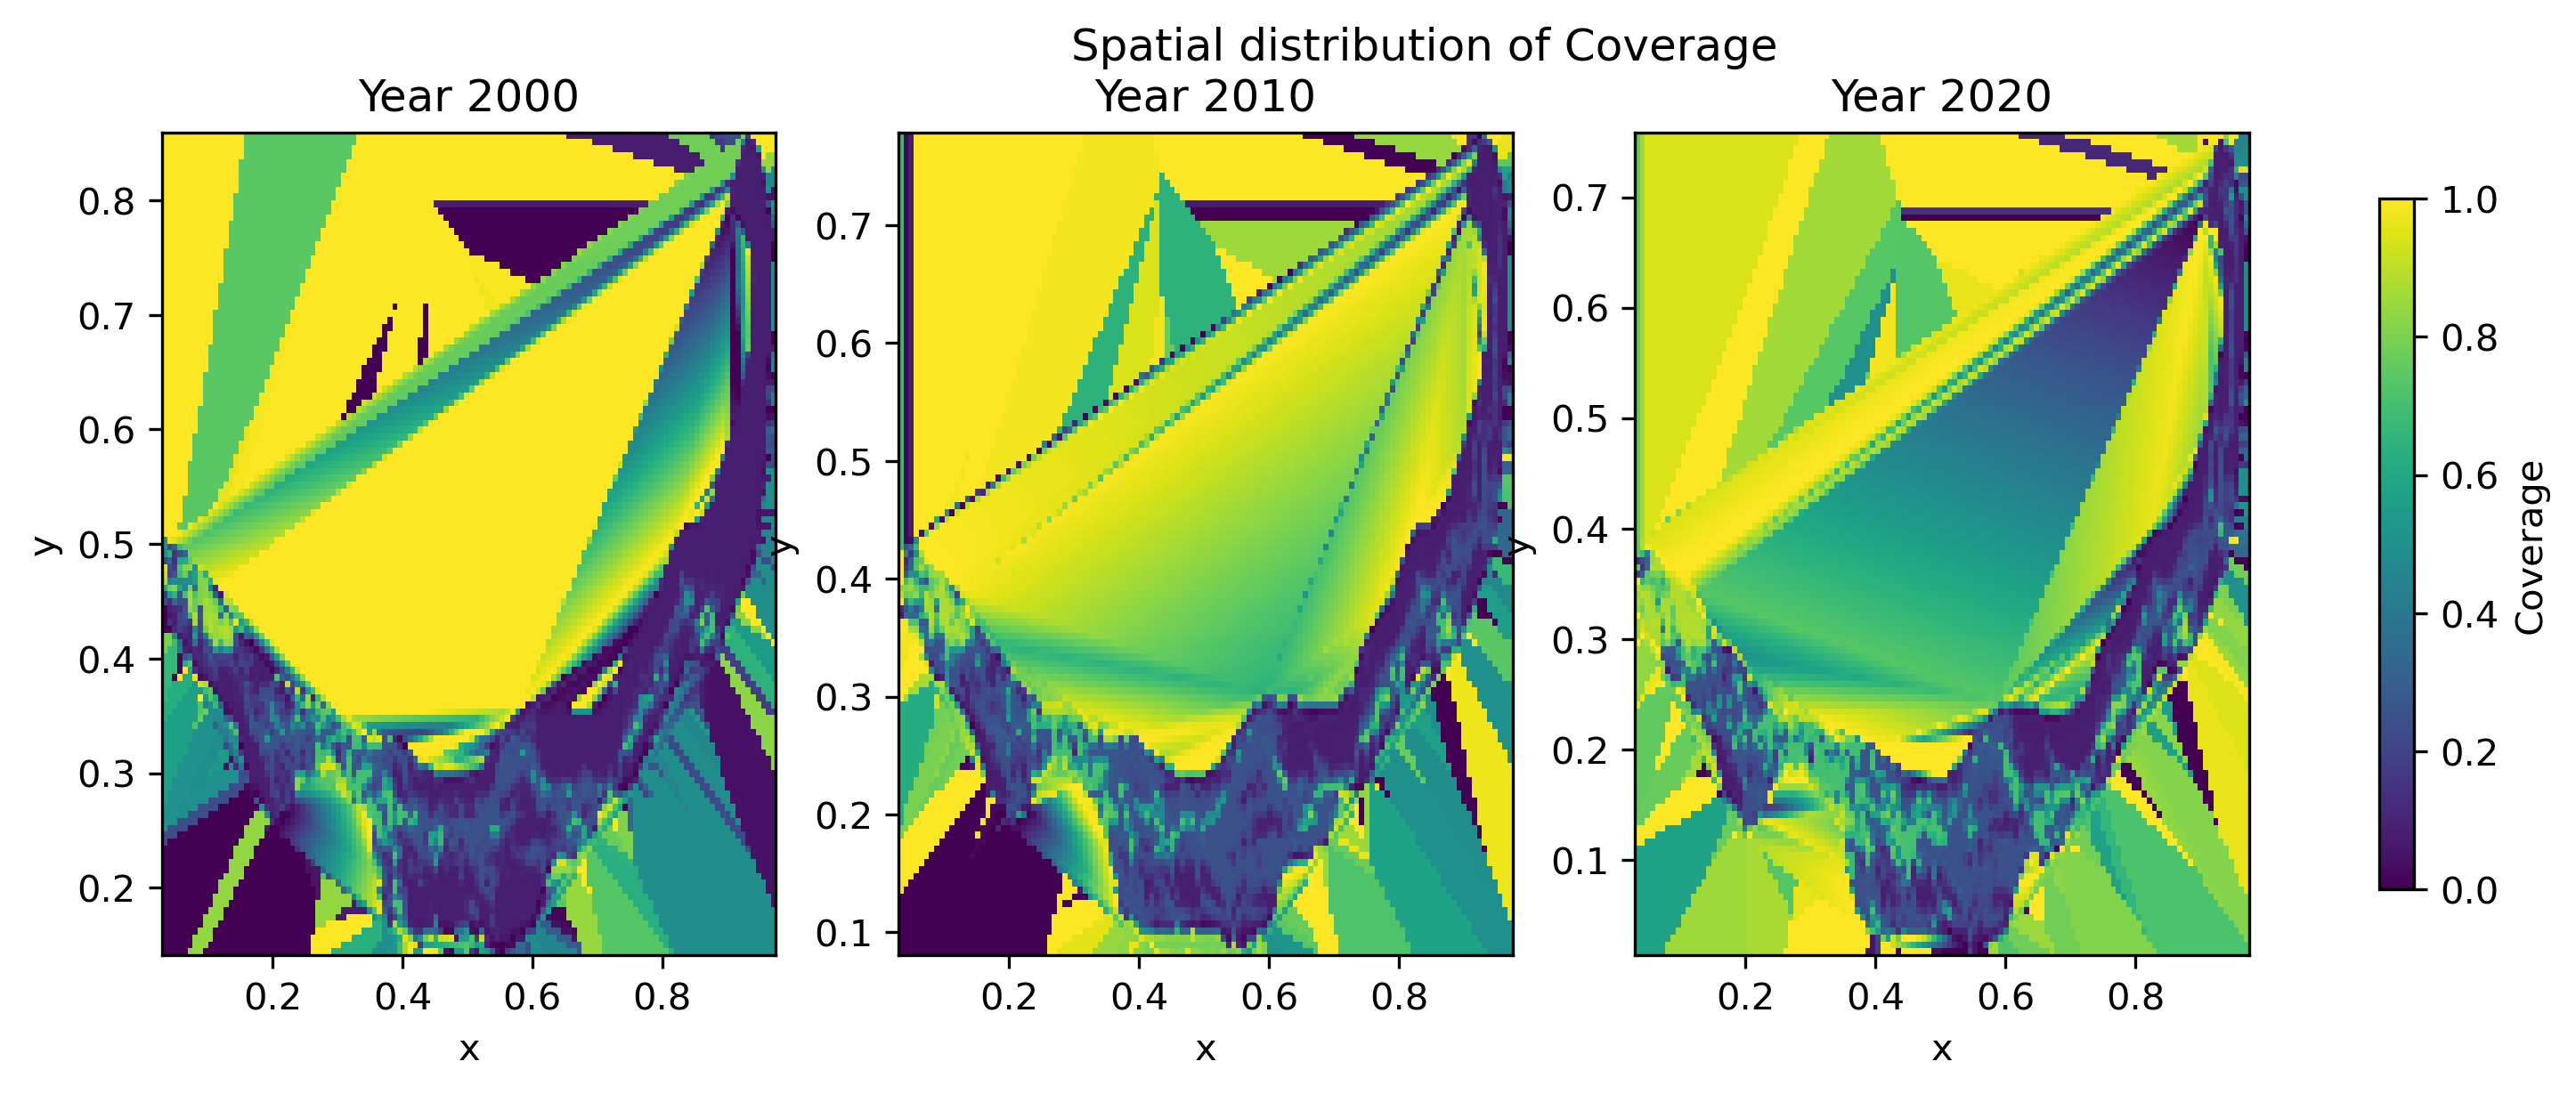
\includegraphics[width=0.85\textwidth]{fig13_spatial_trend.png}
		\caption{Spatial trend of vegetation change from the verification system.}
		\label{fig:spatial_trend_supp}
	\end{figure}
	
	\begin{figure}[H]
		\centering
		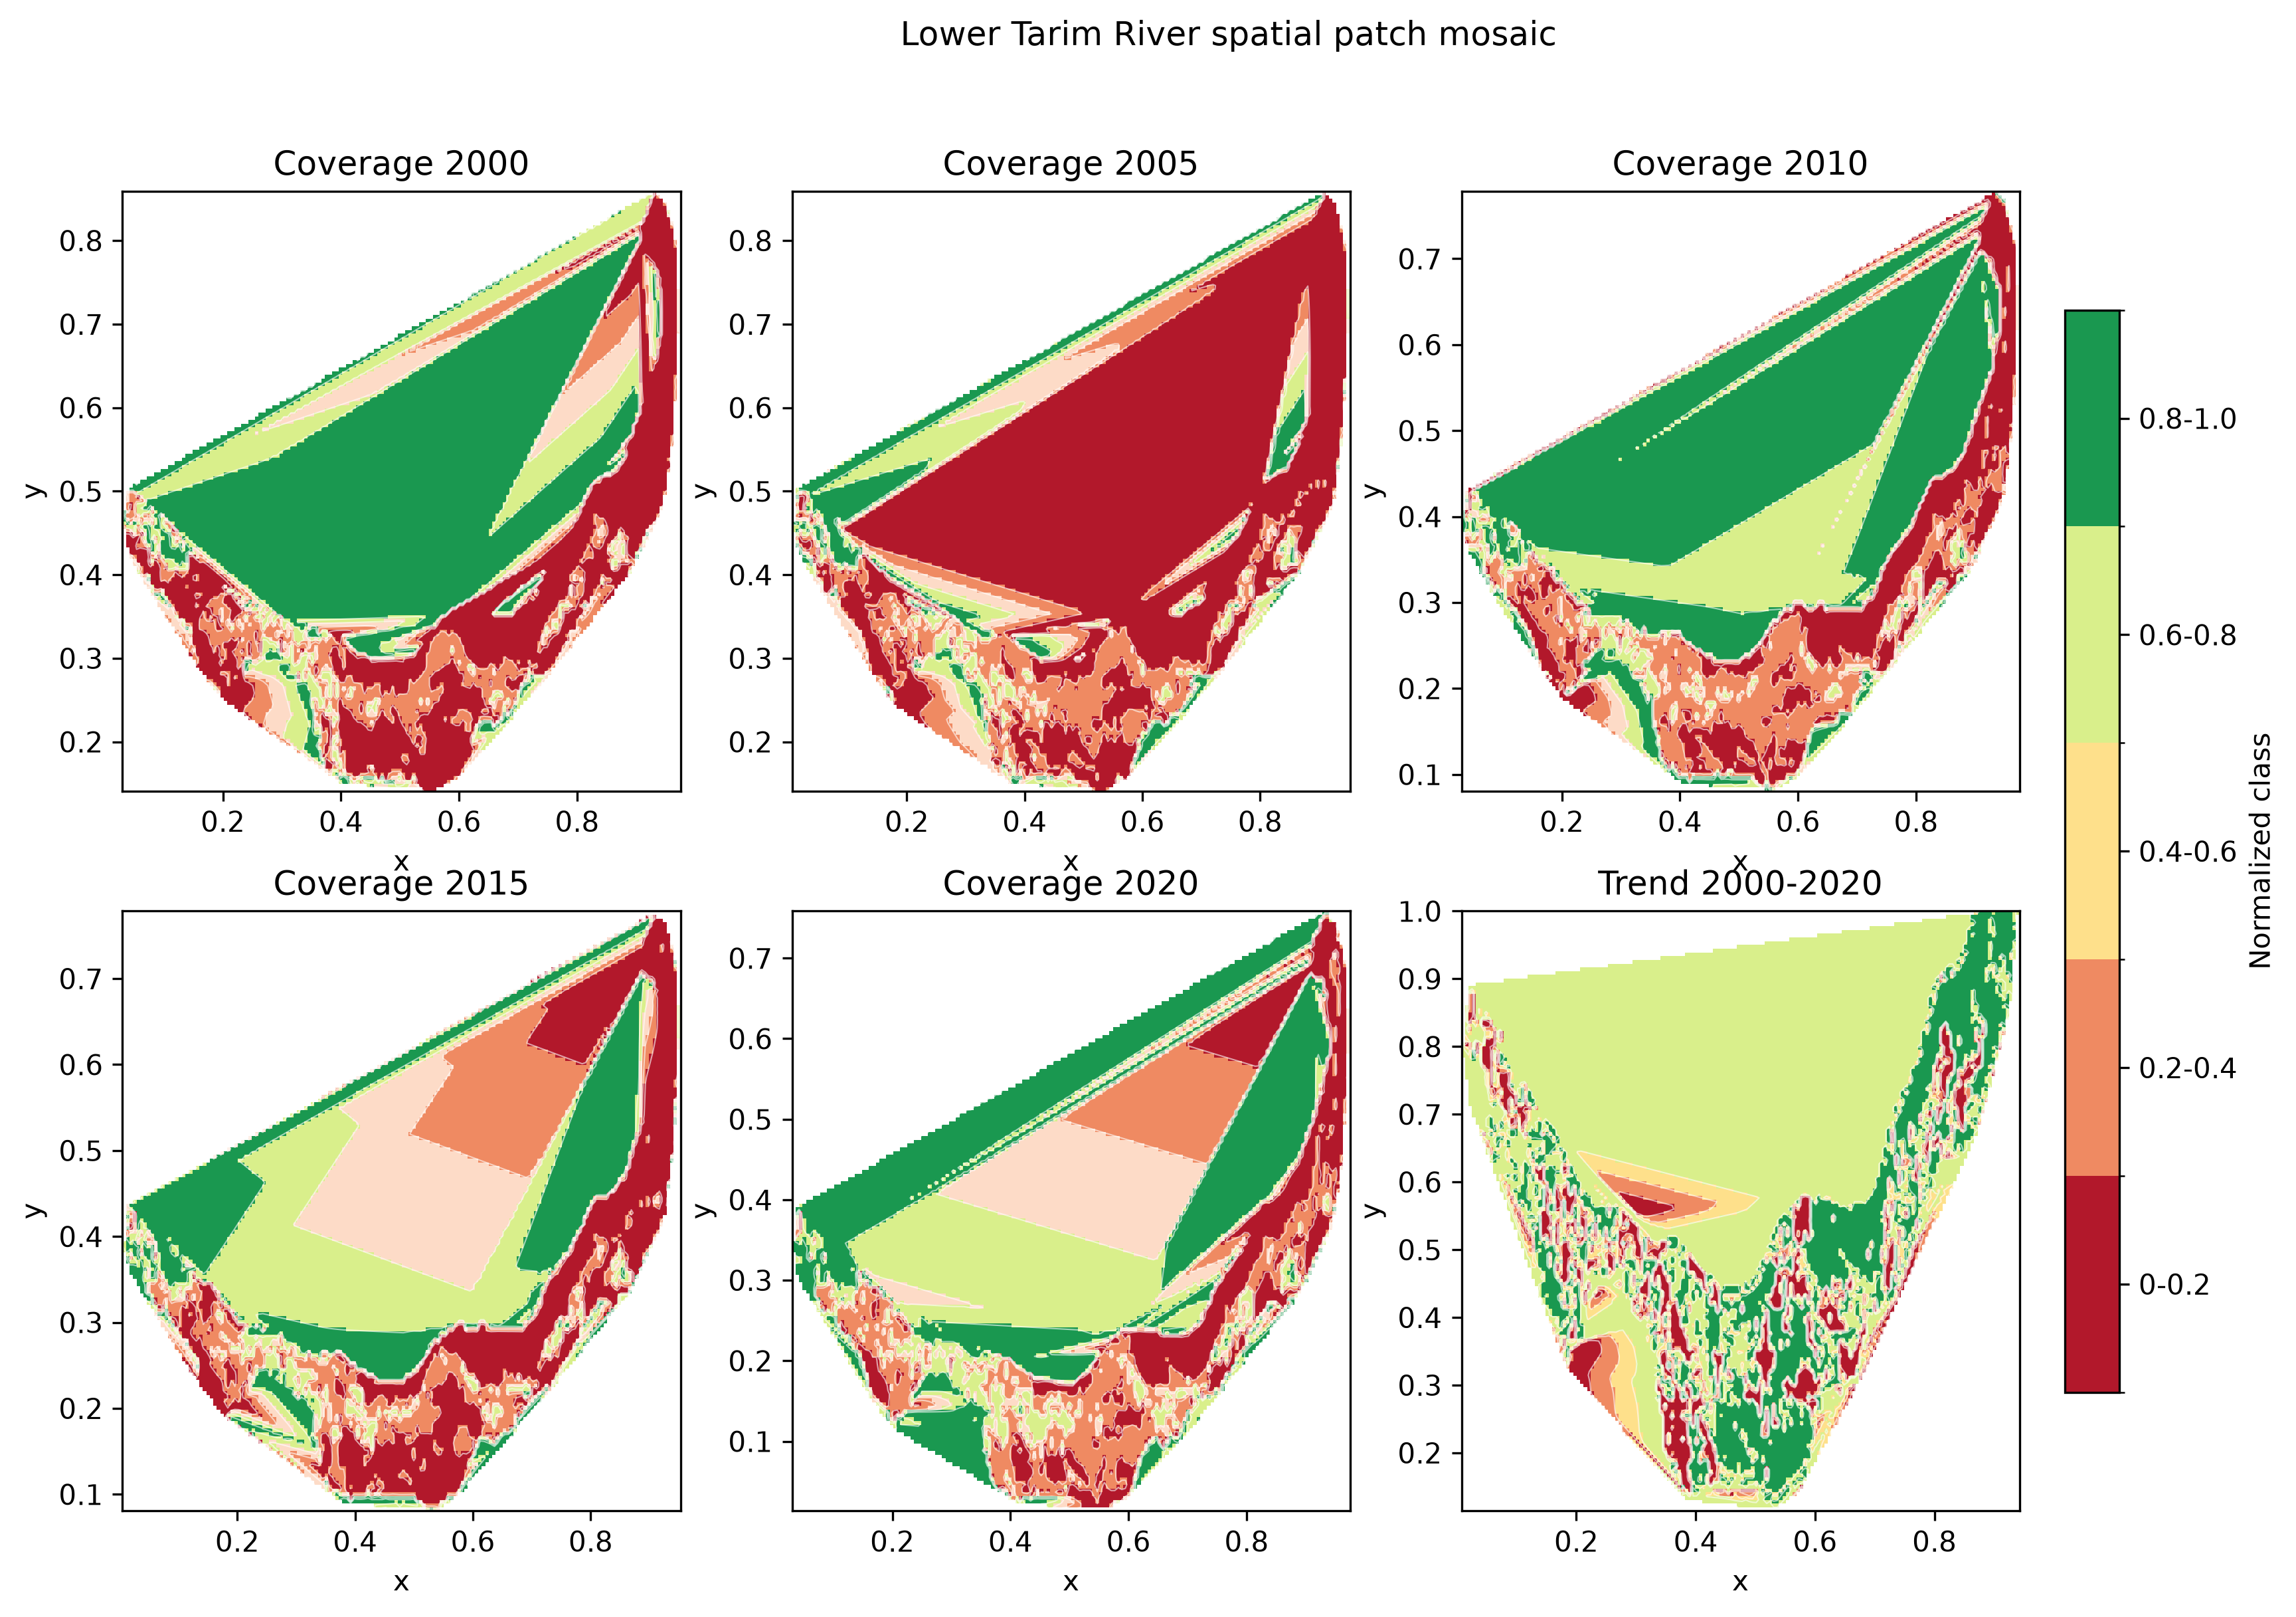
\includegraphics[width=0.85\textwidth]{fig16_spatial_patch_mosaic.png}
		\caption{Spatial patch mosaic showing vegetation pattern organization.}
		\label{fig:mosaic_supp}
	\end{figure}
	
	\subsection{Potential Landscape}
	
	\begin{figure}[H]
		\centering
		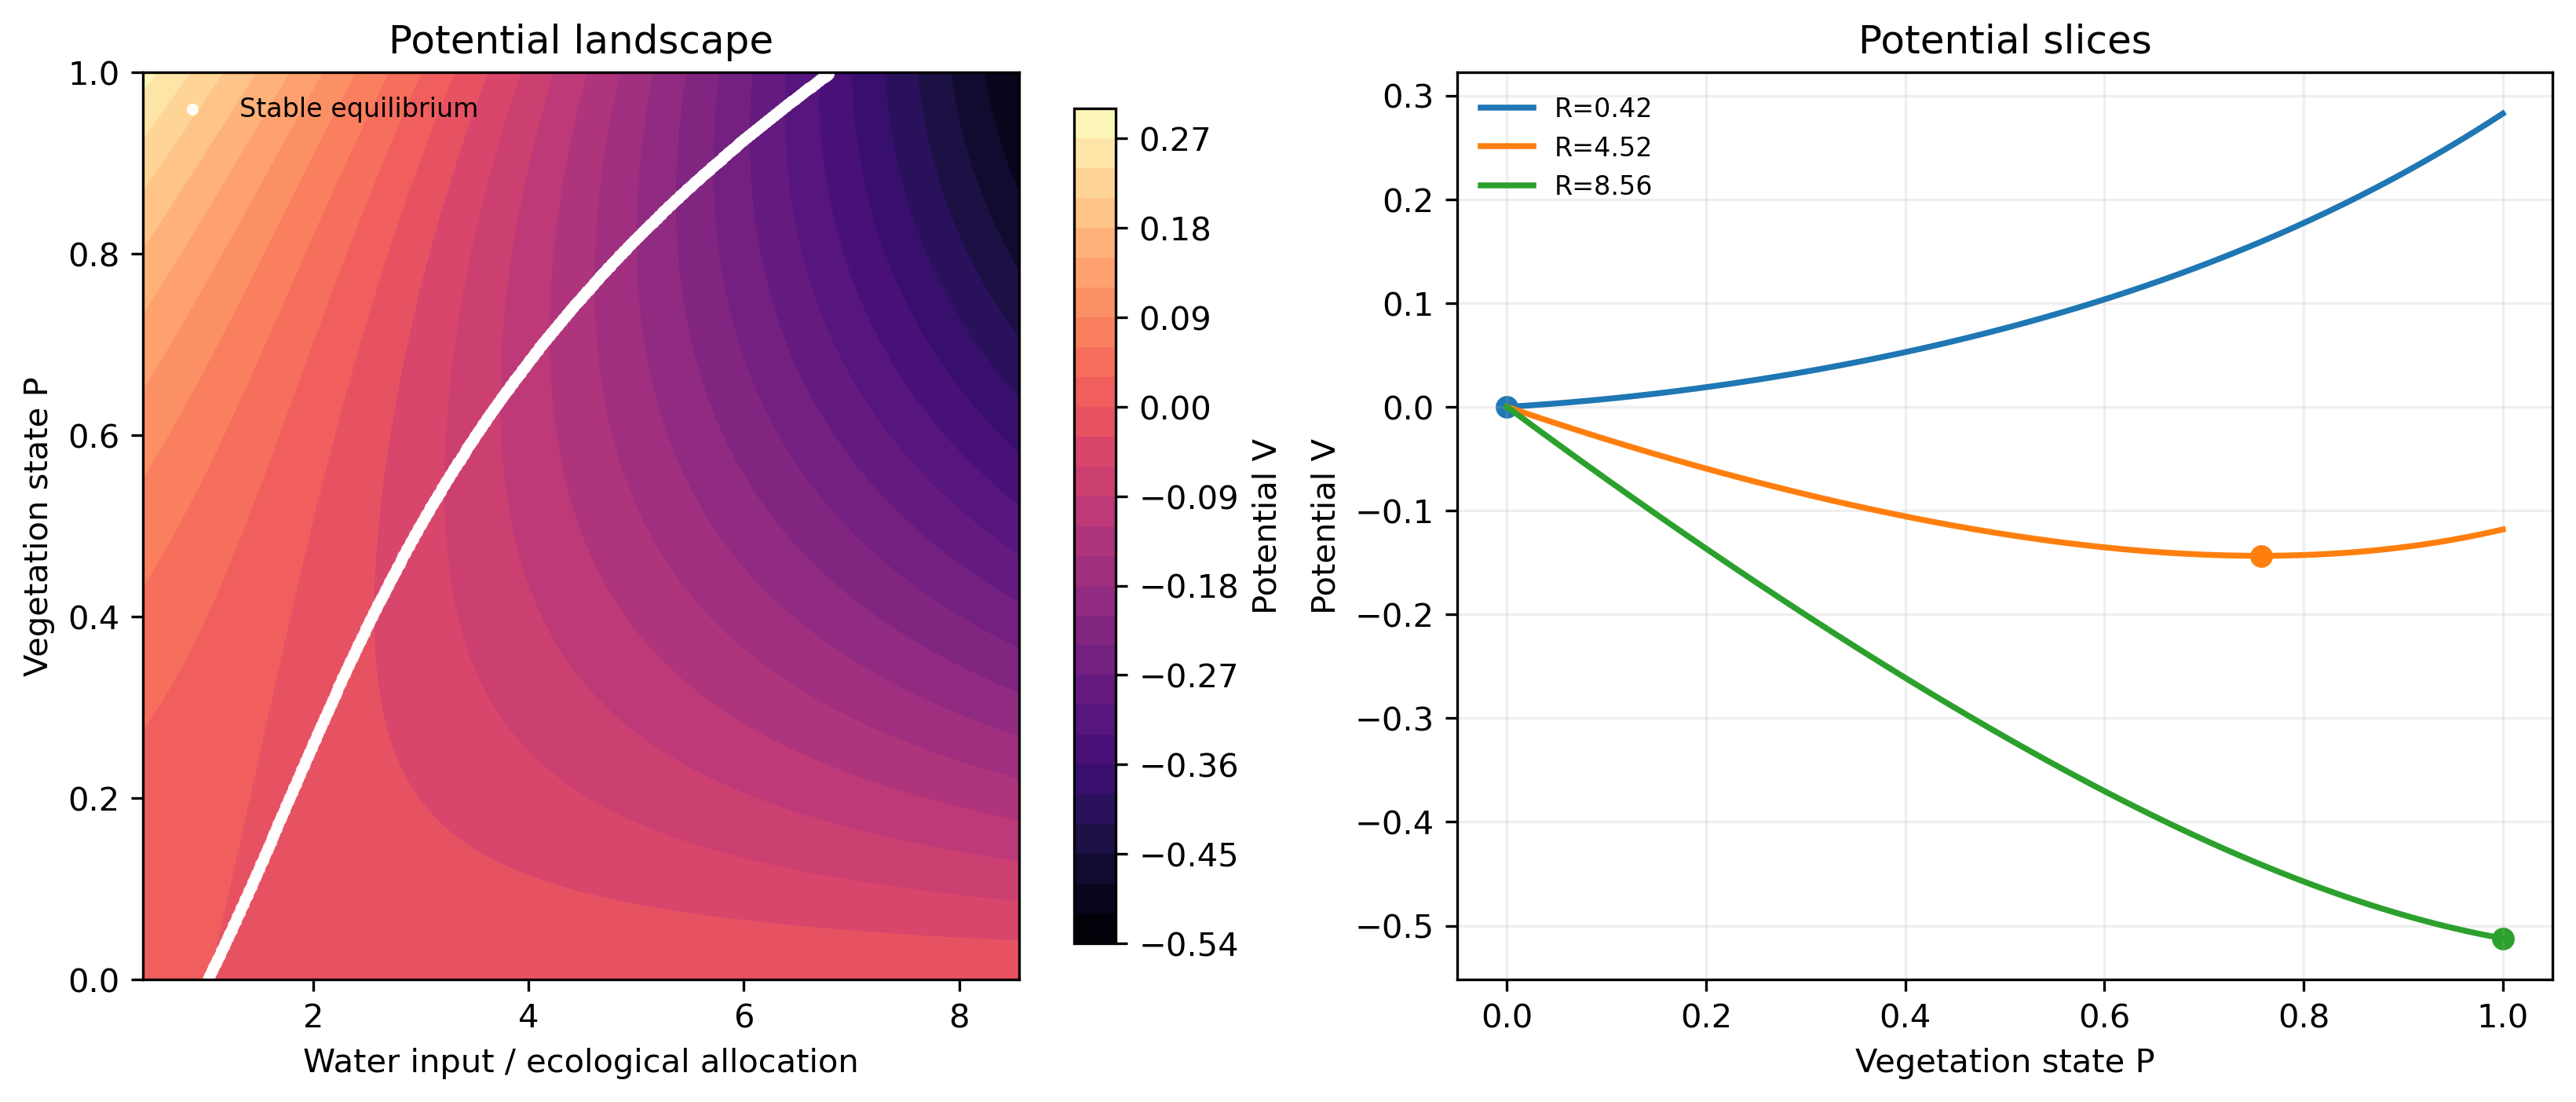
\includegraphics[width=0.85\textwidth]{fig12_potential_landscape.png}
		\caption{Potential landscape at different water input levels. (a) $R=0.42$: desert dominates; (b) $R=4.52$: bistability; (c) $R=8.56$: vegetated dominates.}
		\label{fig:potential_supp}
	\end{figure}
	
	\subsection{Correlation Heatmap}
	
	\begin{figure}[H]
		\centering
		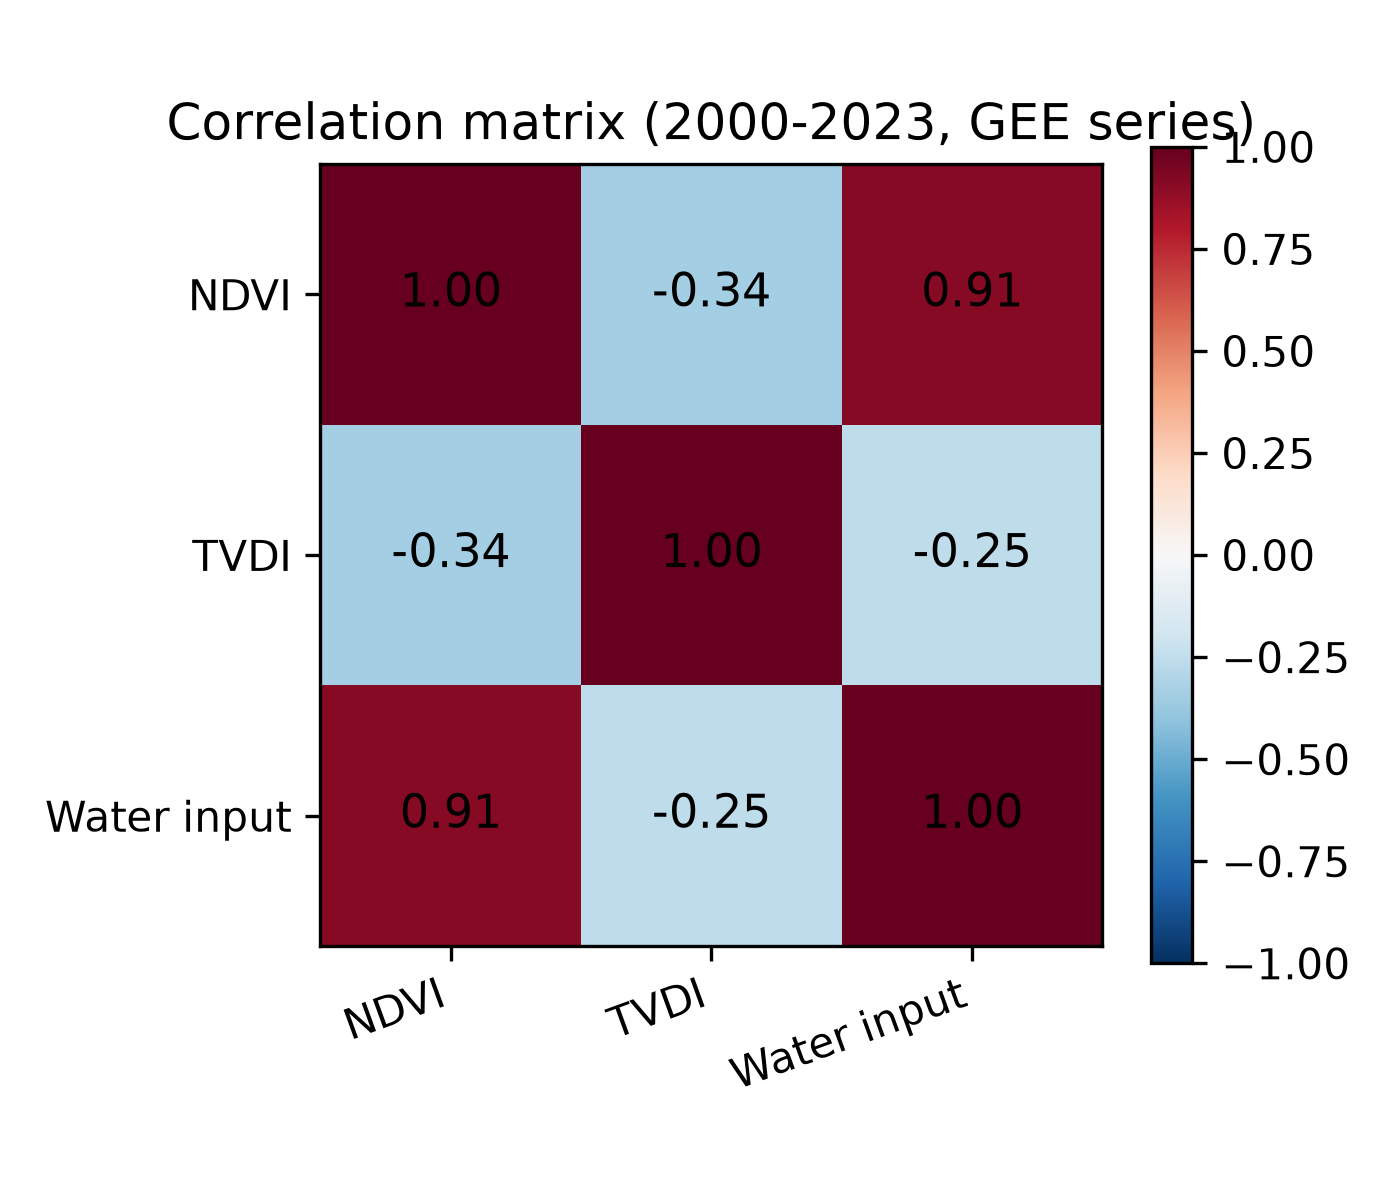
\includegraphics[width=0.6\textwidth]{fig11_correlation_heatmap.png}
		\caption{Correlation heatmap: NDVI-TVDI ($r=-0.99$), NDVI-R ($r=0.98$), TVDI-R ($r=-0.99$).}
		\label{fig:correlation_supp}
	\end{figure}
	
\section{Extended Bifurcation and Sensitivity Analysis of the Exploratory Normal Form}
\label{sec:s4}

This section provides additional details on the exploratory hysteresis scenario generated by the PINN-guided reduced cusp normal form.
\subsection{Normal-Form Construction and Exploratory Fold Points}

The direct equilibrium reduction of the implemented temporal ODE did not yield two fold points within the prescribed search range using the PINN-estimated parameters. Therefore, we constructed a reduced cusp normal form:
\begin{equation}
	\frac{dx}{dt} = x^3 - \alpha x - \beta,
	\label{eq:s4_normal_form}
\end{equation}
where $\alpha$ and $\beta$ are control parameters mapped to the water input and vegetation state, respectively. The mapping was designed to preserve the local stability properties inferred from the PINN-calibrated Jacobian.

Solving the normal-form equilibrium conditions yielded the following exploratory fold-point values:

\begin{table}[H]
	\centering
	\caption{Exploratory fold points from the PINN-guided reduced normal form (normalized scale).}
	\label{tab:fold_supp}
	\small
	\begin{tabular}{@{}l p{3.2cm} p{2.3cm} p{6.4cm}@{}}
		\toprule
		Bifurcation & Normalized water input & Vegetation state & Interpretation \\
		\midrule
		Lower fold & 0.35 & 0.793 & Exploratory degradation threshold in the normal form \\
		Upper fold & 0.65 & 0.207 & Exploratory recovery threshold in the normal form \\
		\bottomrule
	\end{tabular}
\end{table}

The width of the exploratory hysteresis interval is:
\begin{equation}
	\Delta F^{\mathrm{(norm)}} = F_{\mathrm{fold2}}^{\mathrm{(norm)}} - F_{\mathrm{fold1}}^{\mathrm{(norm)}} \approx 0.65 - 0.35 = 0.30,
	\label{eq:s4_hysteresis_width}
\end{equation}
in normalized model units.

\subsection{Reduced-Model Sensitivity Exploration}

	Figure~\ref{fig:sensitivity_supp} explores how the fold geometry of the reduced normal form responds to perturbations in two key parameters mapped from the PINN estimates: $\eta$ (linked to $a_2$) and $\beta_{\mathrm{irr}}$ (linked to $b_2$).

\begin{figure}[H]
	\centering
	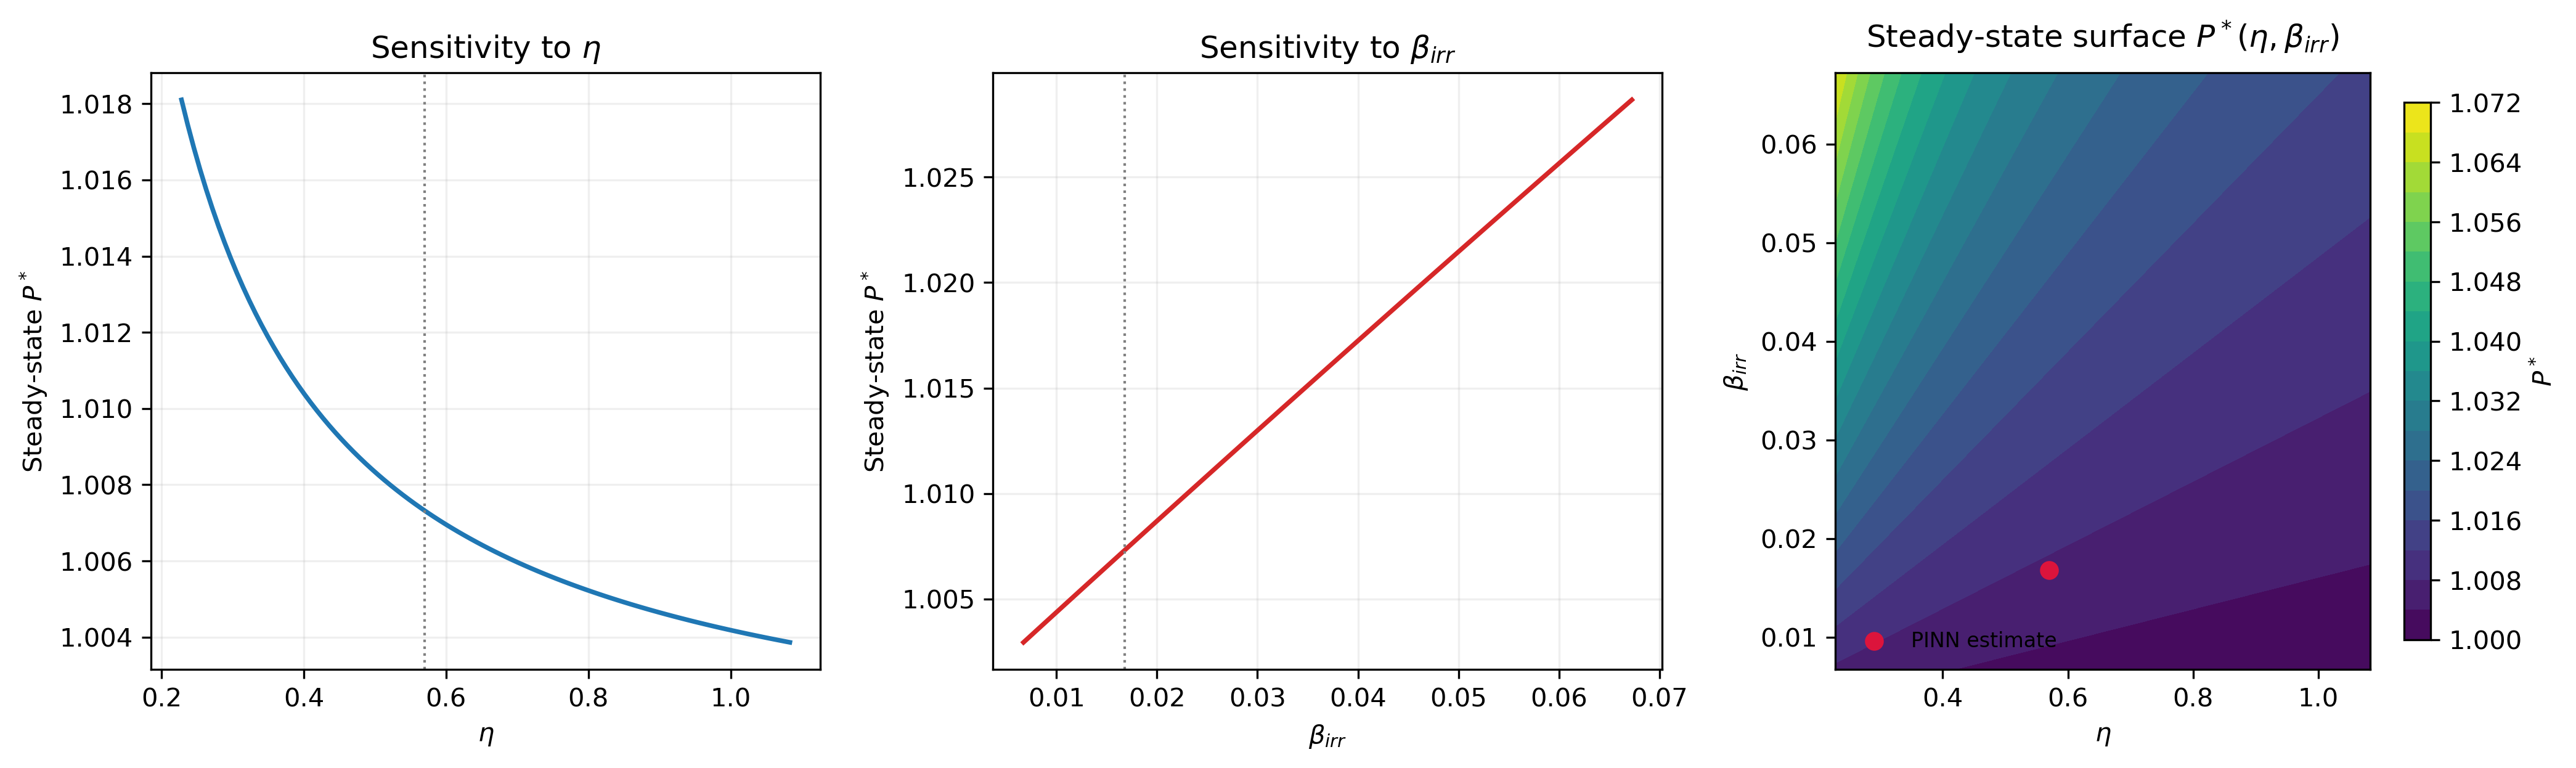
\includegraphics[width=0.85\textwidth]{fig10_parameter_sensitivity.png}
	\caption{Sensitivity exploration of the PINN-guided normal form to perturbations in $\eta$ and $\beta_{\mathrm{irr}}$. The surfaces show how the exploratory fold positions vary under parameter changes, illustrating qualitative uncertainty in the hysteresis scenario.}
	\label{fig:sensitivity_supp}
\end{figure}
	
	\section{Turing Verification: Complete Derivation}
	\label{sec:s5}
	
	\subsection{The Verification System}
	
	The simplified vegetation-water system is:
	\begin{equation}
		\left\{
		\begin{array}{rcl}
			\dfrac{\partial U}{\partial t} &=& r U (U - a)(1 - U) - m U V + D_u \nabla^2 U, \\[0.4cm]
			\dfrac{\partial V}{\partial t} &=& s - q V - c U V + D_v \nabla^2 V.
		\end{array}
		\right.
	\end{equation}
	
	\subsection{Parameter Mapping}
	
	Parameters are mapped from PINN results as follows:
	
	\begin{table}[H]
		\centering
		\caption{Complete parameter mapping}
		\label{tab:mapping_supp}
		\begin{tabular}{lccc}
			\toprule
			Turing Parameter & Symbol & Source & PINN Parameter \\
			\midrule
			Growth rate & $r$ & PINN-guided initialization & 0.7055 \\
			Water loss rate & $q$ & PINN-guided initialization & 0.2517 \\
			Water consumption & $c$ & PINN-guided initialization & 0.1289 \\
			Vegetation equilibrium & $u^*$ & Data-derived & 0.6450 \\
			Water equilibrium & $v^*$ & Data-derived & 0.6880 \\
			Allee threshold & $a$ & Reduced-model search & 0.2949 \\
			Vegetation mortality & $m$ & Computed & 0.0603 \\
			Water supply & $s$ & Computed & 0.2304 \\
			Vegetation diffusion & $D_u$ & Search & $1.0\times10^{-6}$ \\
			Water diffusion & $D_v$ & Search & $1.0\times10^{3}$ \\
			\bottomrule
		\end{tabular}
	\end{table}
	The reduced reaction--diffusion parameters were not obtained through a
	one-to-one mapping of all parameters in the main temporal ODE. Selected
	parameters were initialized from the PINN estimates, whereas the Allee
	threshold and diffusion coefficients were determined by the reduced-model
	search procedure.
	\subsection{Jacobian and Stability}
	
	The Jacobian at equilibrium $(U^*, V^*)$ is:
	\begin{equation}
		J = \begin{pmatrix}
			r (3U^{*2} - 2(1+a)U^* + a) - m V^* & -m U^* \\
			-c V^* & -q - c U^*
		\end{pmatrix}.
	\end{equation}
	
	Stability requires $\tr(J) < 0$ and $\det(J) > 0$.
	
	\subsection{Turing Instability Conditions}
	
	Turing instability occurs when:
	\begin{equation}
		D_v f_U + D_u g_V > 0,
	\end{equation}
	\begin{equation}
		(D_v f_U + D_u g_V)^2 - 4 D_u D_v \det(J) > 0.
	\end{equation}
	
	The unstable wavenumbers satisfy:
	\begin{equation}
		k^2 \in (k_-^2, k_+^2),
	\end{equation}
	where:
	\begin{equation}
		k_{\pm}^2 = \frac{D_v f_U + D_u g_V \pm \sqrt{(D_v f_U + D_u g_V)^2 - 4D_u D_v \det(J)}}{2D_u D_v}.
	\end{equation}
	
	\subsection{Search Procedure for $D_u$ and $D_v$}
	
	The search procedure for diffusion coefficients is:
	\begin{enumerate}
		\item Set $D_u$ in $[10^{-6}, 10^{-2}]$ (log-spaced, 21 values)
		\item Set $D_v$ in $[1, 10^{3}]$ (log-spaced, 31 values)
		\item Retain only pairs that satisfy the classical conditions of Section S5.4
		\item For each retained pair, compute the dispersion relation $\sigma(k)$ on $0\le k\le 60$
		\item Select the pair with the largest positive maximum of $\sigma(k)$
	\end{enumerate}
	
	\begin{table}[H]
		\centering
		\caption{Search ranges and selected values}
		\label{tab:search_supp}
		\begin{tabular}{lcc}
			\toprule
			Parameter & Search Range & Selected Value \\
			\midrule
			$D_u$ & $[10^{-6}, 10^{-2}]$ & $1.0 \times 10^{-6}$ \\
			$D_v$ & $[1, 10^{3}]$ & $1.0 \times 10^{3}$ \\
			$a$ & $(0, 0.645)$ & $0.2949$ \\
			\bottomrule
		\end{tabular}
	\end{table}
	
	\subsection{Numerical Verification of the Linear Prediction}

	For the selected pair ($D_u=10^{-6}$, $D_v=10^{3}$) the conditions of
	Section S5.4 hold, the growth rate is negative at $k=0$, and the unstable band
	is $0.06\le k\le 38.9$ with a maximum $\sigma_{\max}=1.51\times10^{-3}$ at
	$k_{\mathrm{peak}}=1.50$ (wavelength $4.19$ model units). The band is broad,
	so the maximum is shallow and no single wavelength is selected sharply.

	The same equations were integrated on a $128\times128$ lattice with spacing
	$\Delta x=1$ and time step $\Delta t=0.05$, starting from a perturbation seeded
	along the unstable eigenvector at $k_{\mathrm{peak}}$. Over $t=1600$ model time
	units the amplitude of the seeded mode grew at a measured rate of
	$1.52\times10^{-3}$, within $1\%$ of the analytic value, and the power spectrum
	of the final field stayed concentrated at the seeded wavenumber. This verifies
	the numerical implementation of the linear prediction. The saturated nonlinear
	pattern is deliberately not reported: at the calibrated reaction rates
	saturation would require several thousand model time units, over which the
	mortality term drives part of the domain towards extinction rather than towards
	a stationary Turing state. Outputs are archived in
	\texttt{results\_v4/turing\_linear\_check.npz} and the figure is produced by
	\texttt{turing\_linear\_check.py}.

	\section{Data Tables}
	\label{sec:s6_data}
	
	\subsection{Annual Series (2000--2023)}
\label{sec:s6_tables}

Table~\ref{tab:s2} lists the annual NDVI and TVDI values and Table~\ref{tab:s1} lists the ecological water-transfer record. The water state used by the model is the cumulative conveyed volume; the annual allocation is reported next to it so that the two quantities are not confused.

\begin{table}[H]
	\centering
	\caption{Annual average NDVI and TVDI in the lower Tarim River (2000--2023)}
	\label{tab:s2}
	\begin{tabular}{cccc}
		\toprule
		\textbf{Year} & \textbf{NDVI} & \textbf{TVDI} & \textbf{Source} \\
		\midrule
			2000 & 0.127 & 0.784 & Compiled series \\
			2001 & 0.135 & 0.752 & Compiled series \\
			2002 & 0.142 & 0.731 & Compiled series \\
			2003 & 0.151 & 0.712 & Compiled series \\
			2004 & 0.162 & 0.693 & Compiled series \\
			2005 & 0.173 & 0.675 & Compiled series \\
			2006 & 0.183 & 0.658 & Compiled series \\
			2007 & 0.192 & 0.642 & Compiled series \\
			2008 & 0.202 & 0.627 & Compiled series \\
			2009 & 0.211 & 0.613 & Compiled series \\
			2010 & 0.217 & 0.600 & Compiled series \\
			2011 & 0.225 & 0.587 & Compiled series \\
			2012 & 0.232 & 0.575 & Compiled series \\
			2013 & 0.241 & 0.563 & Compiled series \\
			2014 & 0.249 & 0.552 & Compiled series \\
			2015 & 0.257 & 0.541 & Compiled series \\
			2016 & 0.266 & 0.531 & Compiled series \\
			2017 & 0.275 & 0.521 & Compiled series \\
			2018 & 0.283 & 0.511 & Compiled series \\
			2019 & 0.290 & 0.502 & Compiled series \\
			2020 & 0.320 & 0.470 & Compiled series \\
			2021 & 0.310 & 0.485 & Compiled series \\
			2022 & 0.315 & 0.495 & Trend projection \\
			2023 & 0.305 & 0.488 & Trend projection \\
		\bottomrule
	\end{tabular}
	\caption*{Note: Values are reach-scale growing-season aggregates. Entries carried over from the compiled series are labelled \emph{Compiled series} (medium reliability); entries obtained by extending a fitted trend are labelled \emph{Trend projection} (low reliability).}
\end{table}

\begin{table}[H]
	\centering
	\caption{Ecological water transfer in the lower Tarim River (2000--2023)}
	\label{tab:s1}
	\footnotesize
	\begin{tabular}{ccccc}
		\toprule
		\textbf{Year} & \textbf{Annual allocation} & \textbf{Cumulative transfer} & \textbf{Normalized forcing} & \textbf{Source} \\
		 & ($10^{8}$ m$^{3}$) & ($10^{8}$ m$^{3}$) & & \\
		\midrule
			2000 & 1.02 & 1.02 & 0.000 & TRBA \\
			2001 & 2.53 & 3.55 & 0.028 & TRBA \\
			2002 & 3.21 & 6.76 & 0.064 & TRBA \\
			2003 & 3.45 & 10.21 & 0.103 & TRBA \\
			2004 & 3.82 & 14.03 & 0.145 & TRBA \\
			2005 & 4.15 & 18.18 & 0.192 & TRBA \\
			2006 & 4.23 & 22.41 & 0.239 & TRBA \\
			2007 & 4.36 & 26.77 & 0.288 & TRBA \\
			2008 & 4.52 & 31.29 & 0.338 & TRBA \\
			2009 & 4.78 & 36.07 & 0.391 & TRBA \\
			2010 & 5.03 & 41.10 & 0.448 & TRBA \\
			2011 & 5.21 & 46.31 & 0.506 & TRBA \\
			2012 & 5.47 & 51.78 & 0.567 & TRBA \\
			2013 & 5.86 & 57.64 & 0.632 & TRBA \\
			2014 & 6.12 & 63.76 & 0.701 & TRBA \\
			2015 & 6.35 & 70.11 & 0.772 & TRBA \\
			2016 & 6.58 & 76.69 & 0.845 & TRBA \\
			2017 & 6.82 & 83.51 & 0.921 & TRBA \\
			2018 & 7.05 & 90.56 & 1.000 & TRBA \\
			2019 & 7.28 & 97.84 & 1.081 & TRBA \\
			2020 & 8.52 & 106.36 & 1.176 & TRBA \\
			2021 & 7.35 & 113.71 & 1.259 & TRBA rep.+proj. \\
			2022 & 7.18 & 120.89 & 1.339 & TRBA rep.+proj. \\
			2023 & 7.42 & 128.31 & 1.422 & TRBA rep.+proj. \\
		\bottomrule
	\end{tabular}
	\caption*{Note: TRBA denotes the Tarim River Basin Authority. The cumulative transfer is the forcing supplied to the water-input equation and was normalized with the calibration-period minimum and maximum (1.02 and $90.56\times10^{8}$ m$^{3}$). The 2021--2023 entries are report-plus-trend projections and carry low reliability. No effective-rainfall regression or stochastic recharge term was used in the implemented PINN.}
\end{table}



\subsection{NDVI Processing}

NDVI data were derived from MODIS MOD13Q1 product (250 m resolution, 16-day composite). The preprocessing steps included:

\begin{enumerate}
	\item Cloud masking using the MODIS QA band (pixel reliability $\le$ 1).
	\item Temporal smoothing using the Savitzky--Golay filter (window size = 7).
	\item Growing-season averaging (April--October) to produce annual values.
\end{enumerate}

The complete NDVI time series (2000--2023) is provided in Table~\ref{tab:s2}.

\paragraph{Provenance note.} Annual values in the data tables of Section S6 are
reach-scale growing-season aggregates derived from the MODIS processing
described below. Entries from the compiled series are labelled \emph{Compiled series}; entries
obtained by extending a fitted trend rather than from an independent
observation are labelled \emph{Trend projection} and are assigned low
reliability. The same labelling is applied to the ecological
water-conveyance series, whose final three entries combine annual
basin-authority reporting with a trend projection.
\subsection{TVDI Calculation}

The Temperature Vegetation Dryness Index (TVDI) was calculated from the NDVI-LST feature space following the method of Sandholt et al. (2002):

\begin{equation}
	\mathrm{TVDI} = \frac{T_s - T_{s,\min}}{T_{s,\max} - T_{s,\min}}
\end{equation}

where $T_s$ is the land surface temperature, $T_{s,\min}$ is the wet edge (minimum LST for a given NDVI), and $T_{s,\max}$ is the dry edge (maximum LST for a given NDVI).

\begin{itemize}
	\item \textbf{Data sources:} MODIS MOD11A2 (LST, 1 km, 8-day composite) and MOD13Q1 (NDVI, 250 m).
	\item \textbf{Dry edge:} For each 0.02-wide NDVI bin with at least 50 observations, the 98th percentile of LST was used, followed by a least-squares line fit with one 2-sigma refit pass.
	\item \textbf{Wet edge:} The corresponding 2nd percentile of LST was used for each NDVI bin, with the same line-fitting procedure.
	\item \textbf{Time period:} Growing season (April--October), 2000--2023.
\end{itemize}

The annual TVDI values used in the analysis were obtained from the authors'
MODIS processing using the above parameterization. The published studies cited
in the main text provide regional and methodological context, whereas the
numerical series used for calibration are supplied in Table~S2.

TVDI is an empirical remote-sensing dryness index, not a ground measurement. Its magnitude depends on the annual NDVI--LST edge fits. For the lower Heihe comparison, 3,000 region points were used to fit the edges and an independent set of 3,000 oasis points was used for evaluation in each year. The two point sets had zero coordinate overlap in all 24 years. Annual dry-edge $R^2$ was below 0.10 in 2000, 2003, 2013 and 2022; wet-edge $R^2$ was below 0.30 in 2000, 2003 and 2014. These years are explicitly flagged as higher-uncertainty TVDI values in Table~\ref{tab:s6_ejina_tvdi} and should not be treated as in-situ observations.

\begin{table}[H]
	\centering
	\caption{Annual lower Heihe (Ejina Oasis) TVDI and edge-fit diagnostics. Low edge fits are retained but flagged as higher uncertainty.}
	\label{tab:s6_ejina_tvdi}
	\footnotesize
	\begin{tabular}{cccccl}
		\toprule
		Year & Mean TVDI & NDVI bins & Dry-edge $R^2$ & Wet-edge $R^2$ & Quality flag \\
		\midrule
		2000 & 0.681 & 9 & 0.080 & 0.230 & dry and wet edges low \\
		2001 & 0.698 & 8 & 0.302 & 0.384 & -- \\
		2002 & 0.720 & 11 & 0.439 & 0.344 & -- \\
		2003 & 0.687 & 9 & 0.087 & 0.297 & dry and wet edges low \\
		2004 & 0.690 & 7 & 0.379 & 0.471 & -- \\
		2005 & 0.706 & 8 & 0.491 & 0.679 & -- \\
		2006 & 0.699 & 8 & 0.537 & 0.434 & -- \\
		2007 & 0.663 & 9 & 0.156 & 0.564 & -- \\
		2008 & 0.711 & 8 & 0.412 & 0.698 & -- \\
		2009 & 0.700 & 8 & 0.318 & 0.325 & -- \\
		2010 & 0.688 & 9 & 0.520 & 0.663 & -- \\
		2011 & 0.695 & 9 & 0.114 & 0.604 & -- \\
		2012 & 0.695 & 9 & 0.237 & 0.430 & -- \\
		2013 & 0.669 & 8 & -0.073 & 0.647 & dry edge low \\
		2014 & 0.685 & 8 & 0.415 & 0.271 & wet edge low \\
		2015 & 0.706 & 9 & 0.479 & 0.452 & -- \\
		2016 & 0.672 & 9 & 0.121 & 0.312 & -- \\
		2017 & 0.705 & 10 & 0.123 & 0.609 & -- \\
		2018 & 0.714 & 10 & 0.308 & 0.444 & -- \\
		2019 & 0.688 & 11 & 0.434 & 0.443 & -- \\
		2020 & 0.689 & 9 & 0.255 & 0.640 & -- \\
		2021 & 0.736 & 9 & 0.810 & 0.562 & -- \\
		2022 & 0.700 & 8 & -0.020 & 0.482 & dry edge low \\
		2023 & 0.704 & 8 & 0.440 & 0.641 & -- \\
		\bottomrule
	\end{tabular}
	\caption*{Note: Low flags denote dry-edge $R^2<0.10$ or wet-edge $R^2<0.30$. TVDI is computed from MODIS NDVI and LST and is not a ground observation.}
\end{table}

\begin{table}[H]
	\centering
	\caption{Descriptive cross-basin summary for 2000--2023. Ejina values use the point-consistent oasis sample.}
	\label{tab:s6_cross_basin}
	\small
	\begin{tabular}{@{}lrrrrrr@{}}
		\toprule
		Basin & \multicolumn{2}{c}{NDVI} & Change & Trend & TVDI & Water \\
		\cmidrule(lr){2-3}
		 & 2000 & 2023 & (\%) & (yr$^{-1}$) & mean & years \\
		\midrule
		Lower Tarim & 0.0758 & 0.1141 & +50.5 & +0.0017 & 0.727 & 21+3/24 \\
		Lower Heihe (Ejina) & 0.1322 & 0.1446 & +9.4 & +0.0008 & 0.696 & 11/24 \\
		\bottomrule
	\end{tabular}
	\caption*{Note: The comparison is descriptive. Seasonal windows, footprints and water-accounting systems differ between basins. TVDI is an empirical feature-space index, not an in-situ measurement. The Tarim water count denotes 21 reported or compiled values plus three trend projections; the lower Heihe count denotes 11 available annual release values.}
\end{table}

\begin{table}[H]
	\centering
	\caption{Annual Zhengyixia release used for the lower Heihe descriptive comparison. Missing water years are retained as missing.}
	\label{tab:s6_heihe_water}
	\footnotesize
	\begin{tabular}{cccc}
		\toprule
		Year & Water year & Release ($10^8$ m$^3$) & Reliability \\
		\midrule
		2000 & 2000--2001 & 6.76 & verified \\
		2001 & 2001--2002 & 9.23 & verified \\
		2002 & 2002--2003 & 12.56 & verified \\
		2003 & 2003--2004 & -- & missing \\
		2004 & 2004--2005 & -- & missing \\
		2005 & 2005--2006 & 11.45 & verified indexed \\
		2006 & 2006--2007 & 11.96 & verified indexed \\
		2007 & 2007--2008 & -- & missing \\
		2008 & 2008--2009 & -- & missing \\
		2009 & 2009--2010 & -- & missing \\
		2010 & 2010--2011 & -- & missing \\
		2011 & 2011--2012 & -- & missing \\
		2012 & 2012--2013 & -- & missing \\
		2013 & 2013--2014 & 13.02 & reproduced \\
		2014 & 2014--2015 & 12.78 & reproduced \\
		2015 & 2015--2016 & -- & missing \\
		2016 & 2016--2017 & 15.92 & verified \\
		2017 & 2017--2018 & -- & missing \\
		2018 & 2018--2019 & -- & missing \\
		2019 & 2019--2020 & -- & missing \\
		2020 & 2020--2021 & -- & missing \\
		2021 & 2021--2022 & 13.71 & reproduced \\
		2022 & 2022--2023 & 8.49 & verified \\
		2023 & 2023--2024 & 10.58 & verified \\
		\bottomrule
	\end{tabular}
	\caption*{Note: The year denotes the start of the annual water-scheduling period. Missing values were not interpolated or filled with East Juyan Lake inflow.}
\end{table}

\subsection{Effective Water-Input Construction}

The ecological water-transfer series was first assembled from annual monitoring
records. For PINN calibration, the observed water input was normalized using the
minimum and maximum values during the calibration period:
\begin{equation}
	F(t)=\frac{W(t)-W_{\min}^{\mathrm{cal}}}
	{W_{\max}^{\mathrm{cal}}-W_{\min}^{\mathrm{cal}}}.
\end{equation}

The ecological water-transfer series was normalized using the minimum and
maximum values during the calibration period. No additional effective-rainfall
regression or stochastic recharge term was used in the implemented PINN. The
normalized forcing $F(t)$ was supplied directly to the water-input equation of
the calibrated temporal ODE. The raw water-transfer data and normalization
constants are provided in Table~\ref{tab:s1}.
\section{Additional Comparison and Robustness Results}
\label{sec:s7}

\subsection{Windowed Skill of the Calibrated Model}

Table~\ref{tab:s7_full_holdout} reports the RMSE of the calibrated PINN and of the three reference models in the two evaluation sub-windows, in normalized units so that the variables are comparable. The coefficient of determination is negative for every model in both sub-windows, so RMSE is the quantity used for the comparison; errors in the original units are reported in the main text.

\begin{table}[H]
	\centering
	\caption{RMSE in normalized units for the two evaluation sub-windows. The 2019--2020 window contains two withheld observations and the 2021--2023 window three trend-projected entries.}
	\label{tab:s7_full_holdout}
	\small
	\begin{tabular}{llccc}
		\toprule
		Window & Model & NDVI & TVDI & Water \\
        \midrule
        2019--2020 & Persistence & 0.140 & 0.086 & 0.088 \\
        (2 withheld) & AR(1) free run & 0.095 & 0.052 & 0.007 \\
        & Nonlinear ODE (forward) & 0.256 & 0.228 & 0.173 \\
        & PINN & 0.203 & 0.131 & 0.175 \\
        \midrule
        2021--2023 & Persistence & 0.056 & 0.041 & 0.082 \\
        (3 projected) & AR(1) free run & 0.073 & 0.078 & 0.015 \\
        & Nonlinear ODE (forward) & 0.159 & 0.130 & 0.178 \\
        & PINN & 0.181 & 0.086 & 0.346 \\
        \bottomrule
	\end{tabular}
\end{table}

\subsection{Ablation of the Loss Terms}

The three loss configurations were compared under an identical reduced budget (1500 Adam epochs, 60 LBFGS steps, three seeds) on the same series, and evaluated over the combined 2019--2023 window in normalized units. Table~\ref{tab:s7_ablation} reports the results. The data-only configuration attains the lowest average RMSE, and adding the governing-equation residual does not improve out-of-range transfer. The ablation is a diagnostic of what the physics term delivers, namely a dynamically consistent fitted trajectory and parameter estimates, and not evidence of superior extrapolation.

\begin{table}[H]
	\centering
	\caption{Ablation of the loss terms over the combined 2019--2023 window, in normalized units (mean of three seeds).}
	\label{tab:s7_ablation}
	\small
	\begin{tabular}{lcccc}
		\toprule
		Configuration & NDVI RMSE & TVDI RMSE & Water RMSE & Average RMSE \\
		\midrule
		Data-only & 0.175 & 0.096 & 0.284 & 0.185 \\
		Data + ODE & 0.204 & 0.107 & 0.351 & 0.220 \\
		Full PINN & 0.205 & 0.110 & 0.349 & 0.221 \\
		\bottomrule
	\end{tabular}
\end{table}



As a sensitivity check, joint
multiplicative perturbations of $\pm10$, $\pm20$ and $\pm30\%$ were applied to the eight
calibrated parameters (200 draws per level) and the analytic equilibrium branches of the full
three-dimensional ODE were screened over the interval spanned by the observed normalized water
input ($0.000$--$1.244$). A fold-type candidate was recorded when $\det J$ changed sign along
a continuous branch, and a Hopf-type candidate when the Routh--Hurwitz indicator
$A_1A_2-A_3$ changed sign with $A_1>0$ and $A_3>0$.

\begin{table}[H]
	\centering
	\caption{Parameter-perturbation robustness of the critical-point screen}
	\label{tab:robust_supp}
	\small
	\begin{tabular}{lcccc}
		\toprule
		Perturbation & Draws & Fold crossings in observed range & Hopf crossings & $\min|\det J|$ \\
		\midrule
		$\pm10\%$ & 200 & 0 & 0 & $1.9\times10^{-2}$ \\
		$\pm20\%$ & 200 & 1 (0.5\%) & 0 & $2.3\times10^{-6}$ \\
		$\pm30\%$ & 200 & 6 (3.0\%) & 0 & $5.4\times10^{-7}$ \\
		\bottomrule
	\end{tabular}
\end{table}

No Hopf-type crossing occurred in any of the 600 perturbed parameter sets, so the absence of a
Hopf bifurcation is robust to parameter perturbation within this range. Fold-type crossings
appeared at $\mu\approx0.157$, $0.279$, $0.953$, $0.997$, $1.075$, $1.095$ and $1.174$ in the
seven affected draws. Those locations correspond to normalized water inputs reached between 2016
and 2019 in the observed record. The compiled NDVI series shows no discontinuity at that level.
The nominal parameter set produced no crossing
anywhere in the scanned interval, with $\min|\det J|\approx3.5\times10^{-2}$. All results were
produced by \texttt{bifurcation\_robustness.py} and archived in \texttt{results\_robustness/}.

\subsection{Windowed Skill Summary}

Figure~\ref{fig:skill_supp} summarises the same comparison as a bar chart. Within the calibration window the PINN has the lowest RMSE for NDVI and TVDI, whereas in the combined evaluation window the persistence and AR(1) forecasts are the most accurate for every variable; the two evaluation sub-windows are listed separately in Table~\ref{tab:s7_full_holdout}.

\begin{figure}[H]
	\centering
	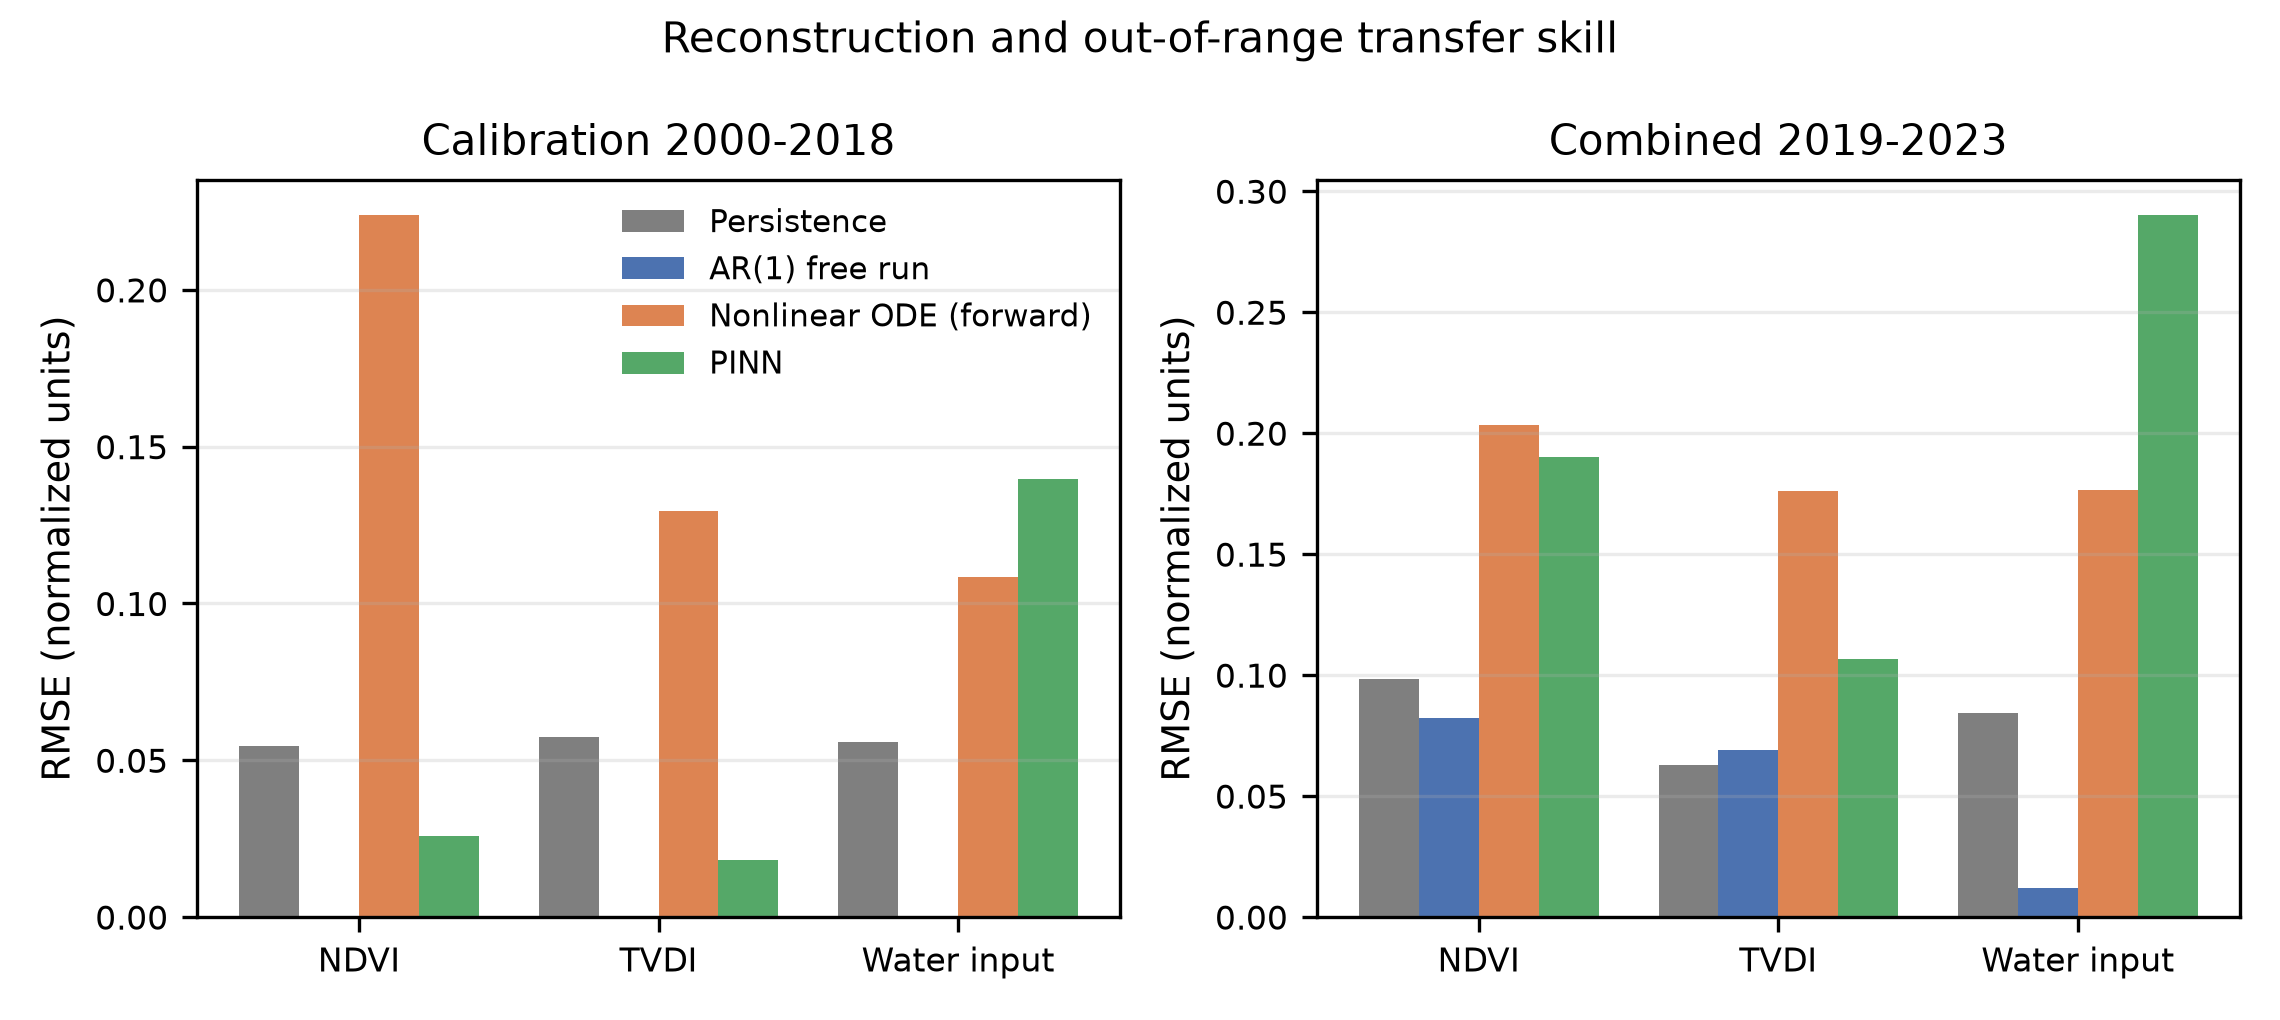
\includegraphics[width=0.95\textwidth]{fig_split_skill.png}
	\caption{RMSE in normalized units over the calibration window and the combined evaluation window (2019--2023). Lower values are better.}
    \label{fig:skill_supp}
\end{figure}
\section{Ten-Metre Spatial Pattern Test: Windows, Holdout Protocol and Per-Window Results}

This section documents the data-facing spatial test summarised in Sections~2.4 and 3.5 of the main text. It is separate from the temporal calibration (Sections S1--S2) and from the reduced Turing verification (Section S5).

\subsection{Window Inventory and Export Settings}

Three fixed windows were exported in EPSG:32645 (WGS~84 / UTM zone 45N) at a 10~m pixel size through Google Earth Engine. The lower-left coordinates are the raster origins reported in the GeoTIFF headers; the mask band accompanying each window was 1 in every retained pixel.

\begin{table}[H]
	\centering
	\caption{Inventory of the three georeferenced analysis windows.}
	\label{tab:s9_windows}
	\small
	\begin{tabular}{lcccc}
		\toprule
		Window & Easting (m) & Northing (m) & Columns $\times$ rows & Ground extent \\
		\midrule
		W1 & 555410 & 4487660 & $129\times128$ & $1.29\times1.28$ km \\
		W2 & 602590 & 4466170 & $129\times129$ & $1.29\times1.29$ km \\
		W3 & 621790 & 4395900 & $129\times128$ & $1.29\times1.28$ km \\
		\bottomrule
	\end{tabular}
\end{table}

\subsection{Data Products and Validity Screen}

The three states of the spatial model are $P$ (normalised Sentinel-2 NDVI), $T$ (TVDI from the co-registered NDVI--LST feature space) and $R$ (normalised Sentinel-2 NDWI). Landsat 8/9 surface temperature has a 100~m native footprint and was resampled to the 10~m grid; it is therefore a 10~m analysis grid with 100~m thermal support, not a 10~m thermal observation. TVDI derived from it inherits the same limitation and is not a ground measurement.

Two years required an explicit decision. The 2015 exports contained valid thermal data but no valid Sentinel-2 NDVI or NDWI (valid fraction 0 in all three windows), so 2015 was excluded from the pattern test rather than gap-filled. The 2016 exports use Sentinel-2 top-of-atmosphere reflectance rather than surface reflectance and were retained only as low-reliability supporting data. The primary calibration window was therefore 2017--2021, with 2022--2023 withheld in full.

\subsection{Holdout Protocol and Pass Criteria}

The network was formulated as a persistence-anchored residual model,
\begin{equation}
	X(x,y,t)=X(x,y,2021)+\frac{t-2021}{t_s}\,\epsilon\,[2g_{\theta}(x,y,t)-1],
	\label{eq:s9_residual}
\end{equation}
with $t_s=4$ years and $\epsilon=0.2$; the residual vanishes identically at the 2021 anchor. The loss combined raster observations, three reaction--diffusion residuals, zero-flux boundary conditions and the initial-condition constraint. The unanchored spatiotemporal PINN, trained with the same budget and split, was retained as a negative control.

Two independent criteria were applied. A pattern-level pass required a radial spectral cosine $\ge0.95$, a detrended pixel correlation $\ge0.5$, and a pixel correlation at least $0.2$ above a random-phase null constructed from the same power spectrum. An absolute-level pass required $R^2\ge0.5$ for $P$ and $R$; $T$ was evaluated but is reported as a diagnostic state only.

\subsection{Absolute-Level Holdout Accuracy}

\begin{table}[H]
	\centering
	\caption{Absolute-level holdout accuracy of the persistence-anchored residual spatial PINN, per window and year. Values are in normalised units defined by the 2017--2021 calibration period.}
	\label{tab:s9_absolute}
	\small
	\begin{tabular}{llcccc}
		\toprule
		Window & Year & State & RMSE & MAE & $R^2$ \\
		\midrule
		W1 & 2022 & $P$ & 0.054 & 0.039 & 0.950 \\
		W1 & 2022 & $T$ & 0.123 & 0.109 & $-2.08$ \\
		W1 & 2022 & $R$ & 0.079 & 0.055 & 0.890 \\
		W1 & 2023 & $P$ & 0.062 & 0.049 & 0.928 \\
		W1 & 2023 & $T$ & 0.162 & 0.125 & $-25.57$ \\
		W1 & 2023 & $R$ & 0.105 & 0.091 & 0.765 \\
		\midrule
		W2 & 2022 & $P$ & 0.060 & 0.041 & 0.959 \\
		W2 & 2022 & $T$ & 0.262 & 0.248 & $-3.17$ \\
		W2 & 2022 & $R$ & 0.074 & 0.052 & 0.940 \\
		W2 & 2023 & $P$ & 0.104 & 0.077 & 0.834 \\
		W2 & 2023 & $T$ & 0.618 & 0.606 & $-21.64$ \\
		W2 & 2023 & $R$ & 0.118 & 0.090 & 0.791 \\
		\midrule
		W3 & 2022 & $P$ & 0.113 & 0.084 & 0.800 \\
		W3 & 2022 & $T$ & 0.411 & 0.403 & $-51.18$ \\
		W3 & 2022 & $R$ & 0.242 & 0.214 & $-0.03$ \\
		W3 & 2023 & $P$ & 0.089 & 0.069 & 0.863 \\
		W3 & 2023 & $T$ & 0.333 & 0.324 & $-43.35$ \\
		W3 & 2023 & $R$ & 0.190 & 0.168 & 0.331 \\
		\bottomrule
	\end{tabular}
\end{table}

The archive \texttt{residual\_multiwindow\_metrics.csv} reports the same quantities together with the persistence and climatology baselines. Those baseline columns use the archived per-window reference fields and are therefore not numerically interchangeable with the calibration-period normalisation used here.

\subsection{Pattern-Level Results}

\begin{table}[H]
	\centering
	\caption{Pattern-level holdout metrics per window and year. $\lambda$ is the dominant radial wavelength of the predicted field and $\lambda_{\mathrm{obs}}$ that of the observed field. The null column is the pixel correlation obtained after randomising the phase of the predicted field.}
	\label{tab:s9_pattern}
	\small
	\setlength{\tabcolsep}{4pt}
	\begin{tabular}{llcccccc}
		\toprule
		Window & Year & State & Spectral cosine & Pixel corr. & Null corr. & $\lambda$ (m) & $\lambda_{\mathrm{obs}}$ (m) \\
		\midrule
		W1 & 2022 & $P$ & 0.999 & 0.965 & 0.034 & 1122 & 1122 \\
		W1 & 2022 & $T$ & 0.983 & 0.347 & $-0.026$ & 1122 & 1122 \\
		W1 & 2022 & $R$ & 0.993 & 0.941 & $-0.028$ & 1122 & 1122 \\
		W1 & 2023 & $P$ & 0.995 & 0.965 & 0.031 & 1122 & 1122 \\
		W1 & 2023 & $T$ & 0.945 & 0.158 & $-0.029$ & 1122 & 561 \\
		W1 & 2023 & $R$ & 0.989 & 0.951 & $-0.029$ & 1122 & 1122 \\
		\midrule
		W2 & 2022 & $P$ & 0.999 & 0.975 & 0.036 & 281 & 281 \\
		W2 & 2022 & $T$ & 0.968 & 0.762 & 0.043 & 563 & 1126 \\
		W2 & 2022 & $R$ & 0.995 & 0.964 & $-0.046$ & 281 & 281 \\
		W2 & 2023 & $P$ & 0.994 & 0.948 & 0.038 & 281 & 281 \\
		W2 & 2023 & $T$ & 0.924 & 0.606 & 0.027 & 563 & 563 \\
		W2 & 2023 & $R$ & 0.993 & 0.940 & $-0.045$ & 281 & 281 \\
		\midrule
		W3 & 2022 & $P$ & 0.976 & 0.886 & $-0.012$ & 374 & 374 \\
		W3 & 2022 & $T$ & 0.982 & 0.560 & 0.047 & 561 & 1122 \\
		W3 & 2022 & $R$ & 0.973 & 0.804 & 0.006 & 374 & 374 \\
		W3 & 2023 & $P$ & 0.969 & 0.919 & $-0.014$ & 374 & 374 \\
		W3 & 2023 & $T$ & 0.939 & 0.631 & 0.035 & 1122 & 561 \\
		W3 & 2023 & $R$ & 0.986 & 0.869 & 0.000 & 374 & 374 \\
		\bottomrule
	\end{tabular}
\end{table}

$P$ satisfies both the pattern-level and the absolute-level criteria in all six window-years. $R$ satisfies the pattern-level criterion in all six window-years and the absolute-level criterion in four of six, failing in W3 in both holdout years. For $T$ the spectral cosine remains high while the pixel correlation and the dominant wavelength diverge from the observations, so $T$ is reported as a diagnostic state and is not counted as a validated pattern.

\subsection{Negative Control}

\begin{table}[H]
	\centering
	\caption{Mean holdout skill across W1--W3 for the unanchored standard spatiotemporal PINN and the persistence-anchored residual model. Values are in normalised units.}
	\label{tab:s9_control}
	\small
	\begin{tabular}{llcccc}
		\toprule
		Year & State & Standard RMSE & Standard $R^2$ & Anchored RMSE & Anchored $R^2$ \\
		\midrule
		2022 & $P$ & 0.286 & $-0.188$ & 0.075 & 0.903 \\
		2022 & $R$ & 0.292 & $-0.292$ & 0.132 & 0.601 \\
		2023 & $P$ & 0.291 & $-0.442$ & 0.085 & 0.875 \\
		2023 & $R$ & 0.282 & $-0.438$ & 0.138 & 0.629 \\
		\bottomrule
	\end{tabular}
\end{table}

The unanchored network fitted its calibration years but drifted during the holdout, producing negative $R^2$ for both $P$ and $R$ in both years. This control is the reason the anchored formulation is used, and it is also the reason the spatial result is described as pattern-level evidence rather than as a spatial forecast.

\subsection{Reproduction}

\begin{sloppypar}
The windows were exported with \texttt{sentinel2\_pattern\_export\_v2.js}. Quality control and training used \texttt{check\_spatial\_windows.py} and \texttt{spatial\_pinn.py}. Pattern scoring used \texttt{assess\_spatial\_pattern.py}, and \texttt{summarize\_spatial\_pinn.py} wrote the summary tables. All outputs are archived under \texttt{results\_spatial\_pinn/}.
\end{sloppypar}

\section*{Code Availability}


The code for data preprocessing, PINN calibration, full-system equilibrium
continuation, bifurcation screening, reduced reaction--diffusion verification,
and spatial-pattern analysis is available with the processed data, result
tables, and figure files in the \href{https://github.com/PangYingxin-max/lower-tarim-pinn/tree/v1.0.1}{GitHub repository snapshot v1.0.1}.
The repository includes the Google Earth Engine export scripts and links to the
original satellite data catalogs; raw satellite scenes are not redistributed.

\bibliographystyle{elsarticle-num}
\bibliography{myrefs}
\end{document}
